% !TEX program = xelatex
\documentclass[master]{thesis-uestc}

\title{基于深度学习的短文本分类研究}
\author{胡可奇}
\usepackage{listings}
\lstset{breaklines}
\begin{document}

    \begin{chineseabstract}
随着我国信息化建设的不断推进,以及移动互联网的不断发展,
互联网中的信息开始爆炸式的增长,进入了以短文本信息为主的碎片化信息时代。
如何从浩如烟海的信息碎片中准确的获取有用信息,成了学者及商业公司关注的焦点。
本文主要研究了中文短文本分类的相关技术,通过对经典文本分类模型的有效改进,
设计并实现了一个新型的短文本分类模型,并改进了传统词向量训练模型,来实现
适合中文短文本分类的分类网络。本文的主要工作包括了以下几个方面:
\begin{enumerate}
    \item 通过研究传统词向量模型在中文语料上的不足,本文改进了原有的训练模型,引入
    了中文汉字信息以及偏旁部首信息,让词向量模型更加适合中文文本,并通过部首转换机制,
    将部首替换为与其对应的汉字,使得词向量模型能够更好地识别具有语义联系的词语
    ,让具有相似语义的单词能够在向量空间中彼此靠近,性能更优,解释性更强。并且以此为基础提出了
    另一个字向量模型,弥补了分词错误对词向量的影响,为后续的分类模型提供了更加丰富的语义信息。
    \item 本文将卷积神经网络与循环神经网组合使用,引入Attention Model技术,
    设计了一个全新的特征提取网络。
    该网络采用了k-max池化与双向循环神经网络技术,具有更好的特征提取能力,能够有效的识别并提取
    文本数据中的语义特征。通过Attention Model技术,
    网络更加专注分类特征的提取,剔除了无效特征,整体上提升了特征向量质量,
    从而提升分类模型的分类效果。
    
    \item 本文采用双通道的短文本分类模型结构,结合了字向量与词向量的文本数据,
    从两个不同的文本表示中对同一段文本提取文本特征,
    极大的丰富了输入短文本的文本信息,有效提升了分类效果,
    并通过与其他同类模型的对比实验,证明了模型的可行性。
\end{enumerate}


\chinesekeyword{短文本,文本分类,深度学习,Attention技术,词向量}
\end{chineseabstract}



\begin{englishabstract}
With aaa

\englishkeyword{time-domain electromagnetic scattering, time-domain integral equation (TDIE), marching-on in-time (MOT) scheme, late-time instability, plane wave time-domain (PWTD) algorithm}
\end{englishabstract}
    
    
    \thesistableofcontents
    \thesischapterexordium
\section{研究工作的背景与意义}

随着信息化进程的不断推进,我国互联网市场空前繁荣。从WEB2.0时代开始,
到如今的“互联网+”时代,互联网已经融入了人们的生活中,也对各行各业产生了深远的影响。
根据中国互联网络信息中心发布的《第40次中国互联网络发展状况统计报告\footnote{\url{http://www.cnnic.net.cn/hlwfzyj/hlwxzbg/hlwtjbg/201708/P020170807351923262153.pdf}}》显示,
截止到2017年6月,我国网民规模达到7.51亿,其中手机网民更是达到7.24亿,
占总体网民的96.3\%,使用率排名前三的互联网应用分别是即时通信(92.1\%)、网络新闻(83.1\%)、
搜索引擎(81.1\%),使用率最高的三个app应用则是微信(84.3\%)、QQ(65.8\%)、微博(38.7\%)。
可以明显看出,人们使用互联网以及获取信息的方式,已经从以前的桌面台式电脑,
转变为移动端的手机、IPAD等掌上设备。

移动设备的盛行,使得人们发布和接收信息都更加方便,
据统计,在2012年,微博用户已经增长到3.68亿,其中69\%通过移动设备登陆,
每天能产生1.17亿条微博。手机用户的大量增加,让互联网信息爆炸式增长,
并且产生了大量碎片化的信息,如微博、QQ说说、留言、商品评论等。据有关部门统计,互联网全体文本信息中,
80\%以上属于内容较少的短文本信息。

如果能够有效分析这些短文本,对其进行精确的分类,可以方便用户有效的梳理这些浩如烟海的文本并掌握对自身有用的信息,
商家也能够根据信息的分类提供更加优质的服务。
例如,内容提供商,如新浪微博、知乎等,可以对其提供的信息进行分类,让用户快速获取自己感兴趣的某一类信息,
同时商家也可以统计用户浏览过的信息类,精确投放用户感兴趣的广告,减少无关广告对用户体验的伤害;
政府相关部门可以根据一段时间内大众发布的微博或朋友圈等信息,掌握当前的热门话题、集中关注点,
监控当前的社会舆情;电子商务平台,如淘宝、京东等,可以利用情感分类技术,提取商品的正面评论与负面评论给用户,
让用户能够更好的筛选与判断优质商品。

但是和传统文章相比,短文本过于短小(通常在100字以内,一般是一句话的长度),
不能提供足够的词共现(word co-occurrence)或上下文,以至于很难从中提取出有效的文本特征\citing{song2014short}。
因此,常规机器学习技术与文本分类算法很难直接应用在短文本之上。那么如何准确高效的对短文本进行分类,
成为了互联网从业者与互联网技术学者所面临的一个重要难题,其突破也会具有重要的商业价值与使用价值。

\section{国内外研究现状}
随着互联网中短文本信息的增多,短文本分类领域得到了广泛的关注,越来越多的学者投入到短文本分类的研究之中。
但由于短文本短小、信息分散的特性,传统基于词频、词共现的分类方法通常得不到较好的效果,比如贝叶斯方法(Naive Bayes)、
最大熵模型(Maximum Entropy Model)、K-邻近算法(K Nearest Neighbors)以及支持向量机(Support Vector Machines,SVMs)。
因此学者们开始尝试从其他方面来改进短文本分类算法,比如语义分析(sematic analysis)、半监督(semi-supervised)算法和集中模型(ensemble models)。

在语义分析方面,纽约大学的Sarah Zelikovitz等人\citing{zelikovitz2005transductive}通过隐含语义索引算法(Latent Semantic Index,LSI)对短文本的语义分析,将文本中的词映射到潜在语义空间,来捕获文本单词之间的相关性,提升分类效果;
清华大学的Chen等人\citing{chen2011short}通过改进的隐含狄利克雷分布(Latent Dirichlet allocation,LDA)模型,将短文本中的单词与多个粒度的话题相关联,从而拓展短文本特征。

在半监督学习方面,Juan Manuel Cabrera等人\citing{cabrera2013distributional}根据分布式词语表示算法(Distributional Term Representations,DTRs),用半监督的方式统计语料中的文档出现特征以及词语共现信息,形成每个词语的上下文信息,最后强化文本表示,以此来克服短文本处理中长度过短、信息高度分散的难点。

中国科学院自动化研究所的冯晓等人\citing{feng2013chinese}则构造了一种集中学习模型,直接确立短文本实例与某一主题直接的相关性,而不是将短文本表示为权重向量,取得了超过向量空间模型(Vector Space Model,VSM)的效果。

随着神经网络与深度学习逐渐兴起,并在计算机视觉、语音识别等领域取得了不错的成果,
越来越多的学者注意到深度学习模型对于特征提取与数据建模上的优势,开始尝试在在自然语言处理问题中引入。而通过神经网络提取出的文本特征向量,可以直接用于其他任务,例如输入传统分类器进行分类。
斯坦福大学的Richard Socher等人\citing{socher2012semantic}构造了一个使用矩阵向量的循环神经网络(MV-RNN),从长度不一致的句子中学习语义信息,
形式长度统一的特征向量,最后放入分类器分类,取得了超过传统文本分类方法的结果;
牛津大学的Nal Kalchbrenner等人\citing{blunsom2014convolutional}提出了动态卷积神经网络(DCNN),利用动态K-max池化的方法,直接获取文本中单词直接的距离关系,避免了对语法分析树的依赖;
哈佛大学的Yoon Kim等人\citing{chen2015convolutional}将动态词向量与预训练好的静态词向量相结合作为同一段文本的两个表示,输入卷积神经网络的两个通道中进行分类,也取得的较好的效果。

但是,随着深度学习使用的逐渐扩大,学者们发现,对于语法复杂、需要分词的中文文本,深度学习模型并不能直接应用,也无法取得英文语料一样的优秀效果。因此,国内学者开始探寻适合中文文本的深度学习模型,也获得了很多不错的成果。

中国科学院自动化研究所的来斯惟等人\citing{lai2015recurrent}设计了一个循环卷积神经网络,在中文长文本分类任务中取得了较好的效果。
纽约大学的张翔等人\citing{zhang2015character}实现了一个字符级别的卷积网络(ConvNets),将中文语句转化为汉语拼音,对中文语料进行分类。
北京大学的李嫣然等人\citing{li2015component}通过在文本表示中引入部首信息,
利用汉字中部首也包含一定语义信息的特点,在连续词袋模型(Continuous Bag-of-Words,CBOW)的基础上,
构造出了一个新的字向量模型,在中文新闻标题分类上获得了明显的效果。

近几年,自然语言处理领域不断发展,一些新的方法也相继出现,2017年,
Google公司开创性的提出注意力(Attention)观点,
认为模型的结果并不是和每一个模型提取出的特征都有密切的关系,
往往一个结果只是由某一个或某几个关键特征所决定的。
这给了学者们新的启示,一些学者于是将注意力观点应用在文本分类之中。
在文献\cite{er2016attention}中,南洋理工大学的Meng Joo Er等人开发的基于注意力池化的卷积神经网络,
利用平行的双向长短期记忆网络构造了一个输入文本的中间向量表示,以此作为卷积神经网络生成的文件特征向量的注意力权重,
最后将经过处理后的文本特征向量输入分类器进行分类;
卡耐基梅隆大学的Zichao Yang等人\citing{yang2016hierarchical}则实现了一个分层注意力网络,整个网络由两层循环神经网络组成,
第一层网络对句子进行建模,经过注意力机制处理之后得到句子的向量表示,
然后第二层根据所有的句子向量得到文章的向量表示,最后根据这个文章向量获得分类结果。

尽管基于注意力机制的文本分类在近几年获得了研究人员的关注并得到了很多成果,但是这些成果大多是基于英文语料的,
如何将该方法推广到其他语言中,并且如何通过注意力机制提升中文文本分类,特别是中文短文本的分类依然是研究人员需要继续的课题。
\section{课题主要内容}
\section{本论文的结构安排}

    \documentclass{standalone}
% preamble: usepackage, etc.
\begin{document}
\chapter{相关技术研究}
随着互联网技术的发展与国民生活水平的提高,手机持有率直线上升,
手机网民大规模增长,人们在网上产生的信息、发布的文本日益碎片化。
为了有效利用这些片段化的信息,短文本分类技术,作为自然语言处理的关键技术之一,
得到了充分的关注与发展,
短文本分类应用的影子在互联网中随处可见。
本章将介绍本文涉及到的相关技术问题。
\iffalse
\section{中文文本分词}
\label{word_seg}
词是最小的能够独立活动的有意义的语言成分,在英文文本中,每个单词天然的由空格分割开来,
使得研究人员可以毫无难度的获取文本中所有的单词,然后进行接下来的研究工作。
但对于中文这样由字组成的连续文本,并不存在这样的语言优势,词语之间没有明确的区分标记,
要想进行语义分析,必须先将中文文本切分,因此中文分词是中文信息处理的基础和关键。
同时,大量实验表明,分词的好坏直接关系着后续分类算法的最终效果,所以选择一个快速并
准确的分词算法尤为重要。目前常用的分词方法主要有两大类:基于字符串匹配的算法与基于规则的算法。
\subsection{基于字符串匹配的分词算法}
基于字符串匹配的分词算法又称为机械分词算法,主要依据外部提供的词典,
按照一定的策略将待切分的中文文本与词典中的词条逐一匹配,
若在词典中找到该词条,则匹配成功并切分为单词,否则做其它相应的处理。
查找词库的匹配策略分为两种:长单词优先的最大匹配法以及短单词优先的最小匹配法。
在实际使用中,人们发现单词切分次数越短,切分出的单词越长,分词效果越好,
所以目前一般使用最大匹配法。
按照匹配顺序的不同,最大匹配算法又可分为:正向最大匹配算法\citing{张劲松2009回溯正向匹配中文分词算法}、
逆向最大匹配算法\citing{李娟2010一种改进的逆向匹配快速切分算法}、
双向最大匹配算法\citing{陈耀东2005基于有向图的双向匹配分词算法及实现}。

(1)正向最大匹配算法

正向最大匹配算法的基本思想是:已知词典中最长单词的长度为$N$,则以$N$最为截取单词初始长度。
对于带切分的中文文本$S$,首先从左向右截取长度为$N$的字符串$W_{1}$,
然后在词典中寻找是否有和该字符串$W_{1}$匹配的单词。如果找到,则将$W_{1}$标记为成功切分出的单词,
再继续从待切分文本的$N+1$处开始下一次匹配;如果没找到,则将截取长度减$1$重新截取,即在$S$的原来位置重新截取长度为$N-1$的字符串,
然后重复之前匹配操作,直到截取长度为$1$。算法流程如图\ref{max_match}所示:

\begin{figure}[h]
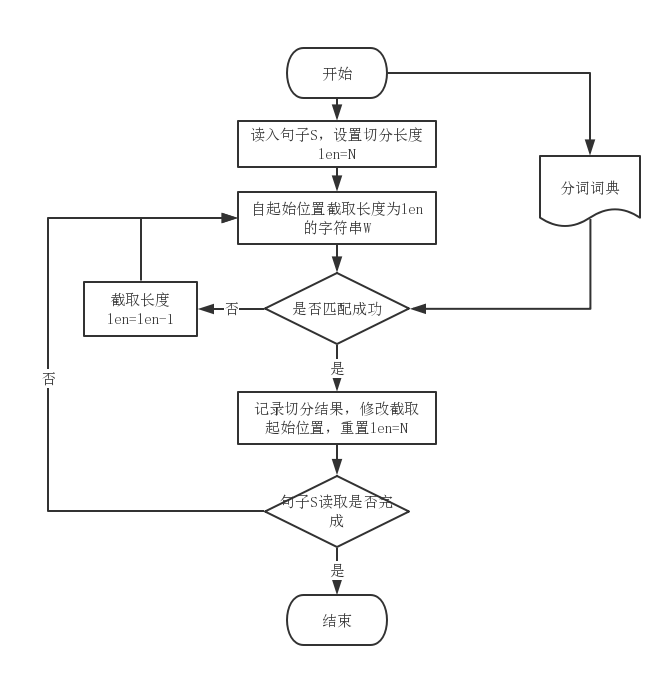
\includegraphics[scale=0.6]{picture/max_match.png}
\caption{正向最大匹配算法流程}
\label{max_match}
\end{figure}

(2)逆向最大匹配算法

逆向最大匹配算法思路和正向最大匹配算法大致相同,不同之处在于截取字符串时的方向由从左向右换成了从右向左。
也就是说,当对句子分词时,根据词典中最长单词的长度,从句子末尾开始向左截取字符串与词典中的
单词匹配,直到切分到句子的开始位置为止。

(3)双向最大匹配算法

双向最大匹配算法是上述两种最大匹配算法的结合,侧重于分词过程中的检错和纠错,其基本思路是对待分词文本分别
采用正向最大匹配和逆向最大匹配进行初步切分,然后将得到的正向分词结果和逆向分词结果进行比较,如果
两种方法的结果一致,则认为分词结果正确,如果结果存在出入,则认为分词存在着切分错误,需要采用其他技术手段消除
结果中的歧义。

从上面的分析可以明显看出,无论哪种最大匹配算法都极度依赖词典,只有在词典覆盖的领域内,才有较理想
的分词效果。对与词典没有覆盖的陌生领域语料,极端情况下甚至会出现单字切分的分词结果。

\subsection{基于统计的分词算法}
\label{n_girm}

这类分词算法并不依赖具体的词典,而是根据语料中的统计信息,识别句子中的单词。即把单词看做是
特定的字的结合,在语料中邻近的字共同出现的次数越多越可能是一个词。所以计算句子中特定字的组合的出现概率,
可以判断这个组合是否是一个词。通过以概率论为理论基础,将中文文本中的每一个词的出现抽象成随机过程,
分词算法不会被待分词文本的内容所影响,对所有领域的中文语料都有统一的效果,
这是极度依赖词典的基于字符串匹配的分词算法所没有优势。根据采用的统计模型不同,基于统计的分词算法
又可分为互信息算法、N元统计模型等。

(1)互信息算法

在概率论和信息论中,两个随机变量的互信息是这两个变量彼此之间依赖性的一个度量。更确切的说,它是根据另一个
随机变量来量化一个随机变量中可以获得的信息量。互信息分词算法是互信息理论在分词中的应用,通过计算
两个相邻字符串的互信息值,来判断它们之间的结合程度(即组成一个单词的可能性)。

对于两个相邻字符串$x$和$y$,它们的互信息值计算公式如下:
\begin{equation}
    I\left ( x,y \right )=\log \frac{p\left ( x,y \right )}{p\left ( x \right )p\left ( y \right )}
\end{equation}

其中$p\left ( x,y \right )$表示字符串$x$和$y$在语料中共同出现的频率,$p\left ( x \right )$与$p\left ( y \right )$分别表示字符串$x$与$y$的出现频率。
当$I\left ( x,y \right )>0$时,表示$x$和$y$具有一定的相关性,并且这个值越大,它们联系的就越紧密,
超过某一个阈值时即可判定为一个词;当$I\left ( x,y \right )=0$时,表示$x$和$y$的关系不明确;当$I\left ( x,y \right )<0$时,表示$x$和$y$直接几乎没有相关性,
基本不会组成一个词。

(2)N元统计模型

N元统计模型又称为N元语言模型(n-gram language model),本质上是对语言建模的一种统计模型。
该模型假定语言满足马尔科夫性,句子中的单词的出现与其前面出现的单词紧密相关,即第$n$个词的出现
只与前面$n-1$个词的出现相关,而和其他任何词都不相关。假设句子$S$由单词序列$\left (w_1,w_2,...,w_m  \right )$组成,
则N元语言模型可表示为:
\begin{equation}
    \begin{aligned}
        P\left ( S \right )&=P\left ( w_1w_2...w_m \right )\\
        &=P\left ( w_1 \right )P\left ( w_2|w_1 \right )...
P\left ( w_i|w_{i-n+1}...w_{i-1} \right )...P\left ( w_m|w_{m-n+1}...w_{m-1} \right )
    \end{aligned}
    \label{n-gram}
\end{equation}

理论上来说,$N$取值越大,模型就越精确,越能揭示出语言的内在结构。但随着$N$的增加,模型的计算复杂度也呈几何式上升,
所以在实际应用中,通常将$N$取值为2、3、4,而$N$取2的N元统计模型称为bigram模型,$N$取3的则称为trigram模型。

在分词应用中,算法首先对句子$S$进行全切分,得到若干分词结果,再根据公式\ref{n-gram}计算这些分词结果的概率$P\left ( S \right )$,
最后选择概率最高的分词结果作为最终结果。


\section{传统文本表示方法}
分词处理之后,文本信息转化为一个单词序列,但对于计算机与程序来说依然是一段没有意义的字符串。
为了让程序能够理解文本信息,继续之后的分类工作,我们需要对其再次处理,提取出其中的有效信息,将字符串文本
映射成结构化的数字信息。

\subsection{向量空间模型}

向量空间模型(Vector Space Model,VSM)最早由Salton等人\citing{薛苏琴2016基于向量空间模型的中文文本相似度的研究}于20世纪70年代提出,
是一种将文本信息表示为向量的代数模型。模型的主要思想是将文本看做单词的简单组合,通过
统计语料中不同单词的个数,构建一个$n$维的向量,向量中每一个纬度都代表一个不同的单词,单词在文本中存在,则此位为$1$,否则为$0$,以此将一段文本信息
转换为一个$n$维的数学向量。

可以明显看出,虽然向量空间模型建立了一个从文本到向量的快速转换,让程序能够容易地对文本进行处理计算,
但这种映射方式太过简单。将文本表示为单词的组合,忽略了词语的位置关系以及词语之间的相互联系。把相同单词都统计为一类,
也忽略了一词多义的情形,让程序难以进行进一步的语义分析。而且,当统计的语料足够多后,
模型产生的向量会拥有一个巨大的维度,造成后续计算的维度灾难。

为了解决上述问题,实际使用中,通常使用文本的关键词作为文本向量,而不是使用所有单词。因此,如何选择关键词就变得尤为重要。


\subsection{TF-IDF特征提取}

TF-IDF(term frequency–inverse document frequency)是一种常用的关键词提取技术,
它表明了一个词对于语料库中一份文本重要程度。算法的中心思想是:一个词的重要性与它在文本中出现的次数成正比,但同时
也与它在整个语料库中出现的次数成反比,即如果某个词在一份文本中出现频率很高,同时在语料库中其他文本中
出现频率很少,那么就认为这个词对于这份文本非常重要。

在TF-IDF中,TF(term frequency)代表词频,对于文本$j$的单词$i$,它的TF值可以通过公式\ref{tf_equ}计算。
\begin{equation}
    TF_{i,j}=\frac{n_{i,j}}{\sum_k n_{k,j}}
    \label{tf_equ}
\end{equation}
其中$n_{i,j}$表示单词$i$在文本$j$中出现的次数,$\sum_k n_{k,j}$表示文本$j$中所有单词的出现次数之和。

IDF(inverse document frequency)代表逆文档频率,是对一个词可以提供的信息量的一个度量,可以体现这个词
在所有文档中是否重要。详细的计算方法如公式\ref{idf_equ}所示。
\begin{equation}
    IDF_{i,D}=\log \frac{\left | D \right |}{1+\left | \left \{ d\in D:t\in d \right \} \right |}
    \label{idf_equ}
\end{equation}
其中$\left | D \right |$表示语料库中的文本总数,$\left | \left \{ d\in D:t\in d \right \} \right |$表示包含单词$i$的文件数量。

最后,根据公式\ref{tf_equ}和\ref{idf_equ}可以得到单词$i$的TF-IDF值,如公式\ref{tf_idf_equ}所示。
\begin{equation}
    TF-IDF_{i,j}=TF_{i,j} \cdot IDF_{i,D}
    \label{tf_idf_equ}
\end{equation}

\subsection{浅层语义分析}
浅层语义分析(Latent Semantic Analysis,LSA)\citing{levy2015improving}是另一种常见的文档建模方法,
该方法认为两个词如果多次出现在同一文档中,则这两个词在语义上具有相似性。基于这一思想,
LSA使用词-文档矩阵(Occurences Matrix)来对文档进行描述,矩阵的一行代表一个单词,
一列代表一篇文档,矩阵中的每个元素则代表该词在文档中出现的次数,
然后通过奇异值分解技术(Singular Value Decomposition,SVD)对矩阵进行降维,
去除矩阵中非必要的信息,最终得到文档的向量表示。


\section{传统文本分类方法}
传统文本分类方法使用机器学习中的分类器对文本特征向量进行分类,这类分类器本质上是
通过设定一个能够将任何特征向量映射到某一具体类别的理想目标函数$\gamma$($\gamma :D\rightarrow C$),
然后根据学习算法减少自身的误差不断接近目标函数,最终实现分类的目的。按照设定的目标函数的不同,
分类器可以分为线性分类器与非线性分类器,下面将对几种常见分类器作简要介绍。
\subsection{贝叶斯分类器}
朴素贝叶斯分类器\citing{mccallum1998comparison}是一种典型的线性分类器,并且也是最古老及最简单的分类器之一。
朴素贝叶斯理论是该分类器的基本理论,它在分类任务中对输入数据有一个基本假设:数据的各特征之间是条件独立的。
虽然这个假设看起来可能明显是错的,但依据朴素贝叶斯理论实现的朴素贝叶斯分类器在结构化或半结构化数据上都有比较理想的表现。
同时,朴素贝叶斯分类器对CPU和内存的消耗也少于其他分类器。

朴素贝叶斯理论是指在上面提到的基本假设下,对于事件$A$和$B$,它们之间的概率关系满足公式\ref{bayes}。
\begin{equation}
    P\left ( A | B\right )=\frac{P\left ( B | A\right )P\left ( A \right )}{P\left ( B \right )}
    \label{bayes}
\end{equation}
而在文本分类任务中,假设一篇文本的特征向量为$D=\left \{ d_1,d_2,...,d_m \right \}$,它的类别为$C$,则上式可以写为公式\ref{bayes_text}。
\begin{equation}
    P\left ( C | D\right )=\frac{P\left ( D | C\right )P\left ( C \right )}{P\left ( D \right )}
    \label{bayes_text}
\end{equation}
其中$P\left ( C \right )$和$P\left ( D \right )$是先验概率(prior probability),分别表示类别$C$和特征向量$D$出现的概率,
$P\left ( D | C\right )$代表在类别$C$中出现特征向量$D$的概率,$P\left ( C | D\right )$则是分类器
的结果,称为后验概率(posterior probability),代表特征向量$D$是类别$C$的概率。实际应用中,
$P\left ( C \right )$和$P\left ( D \right )$以及$P\left ( D | C\right )$都可以根据训练语料库
直接计算得到。

\subsection{支持向量机}
支持向量机(Support Vector Machine,SVM)是感知机的一种改进算法,在机器学习算法中有非常广泛的应用。

在感知机模型中,分类器通过寻找一个可以将数据正确分为两类的超平面来实现二元分类任务。但是,如图\ref{separating_lines}所示,这样的
超平面往往不是唯一,并且不同的超平面选择会导致感知机的分类准确率截然不同。
\begin{figure}[h]
    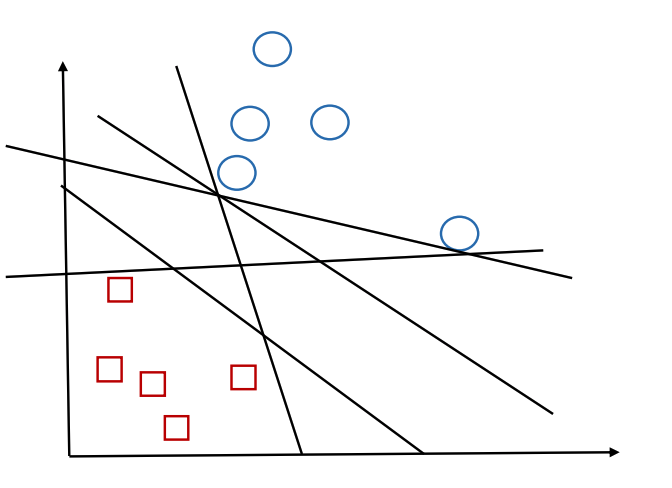
\includegraphics[scale=0.4]{picture/separating-lines.png}
    \caption{超平面示意图}
    \label{separating_lines}
\end{figure}

为了选择一个分类效果最佳的超平面,支持向量机将距离超平面最近的点设定为支持向量,然后让这些支持向量和超平面
之间的距离最大,从而选择出一个最优的超平面,如图\ref{svm}所示。并且对于线性分类不适用的非线性数据(如文本数据),支持向量机利用
核函数的技巧,通过选择一个恰当的转换函数,将非线性数据映射到一个更高维的向量空间当中,让数据重新分布为线性可分的形式。
但是这种做法增加了算法复杂度,复杂的核函数会使算法的计算量成倍的提高,而且如何选择合适的核函数让数据线性可分也没有一个统一
的方法。
\begin{figure}[h]
    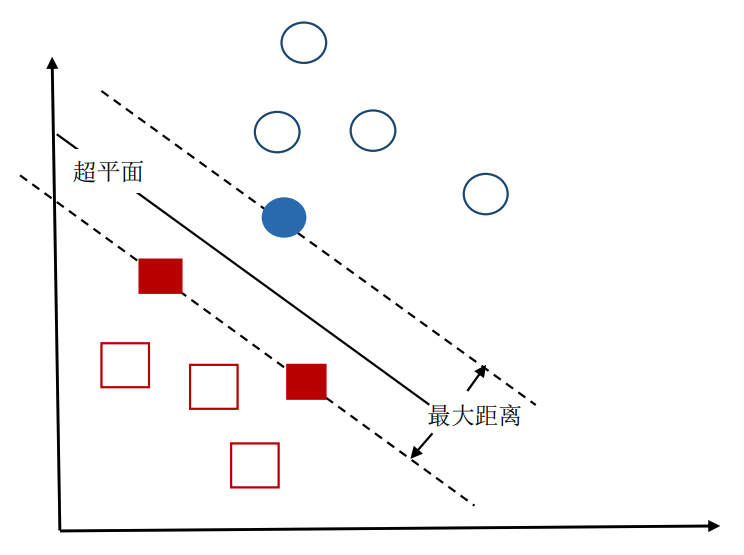
\includegraphics[scale=0.35]{picture/svm.png}
    \caption{支持向量示意图}
    \label{svm}
\end{figure}
\fi
\section{文本表示方法}
文本信息本质上是一个字符序列,
这对于计算机与程序来说就是一段没有意义的字符串。
为了让程序能够理解文本内容,继续之后的分类工作,
我们需要对其进行一定的处理,
将字符串文本映射成结构化的数字信息。
根据处理粒度的不同,文本表示方法可以分类基于词的文本表示方法与最近兴起的基于字(character)
的文本表示方法。
\subsection{基于词的文本表示方法}
在自然语言处理领域,一般都把词看做语言中具有独立语义的最小单元,因此
无论是过去的基于统计特征的传统文本处理算法还是目前火热的深度学习方法,都
把词当做文本的基本组成,并使用它的某种数字形式来表示文本。

目前,基于词的文本表示方法主要有过去的One-hot表示法以及现在常见的分布式表示法,下面
对这两种方法进行介绍。

(1)词的One-hot表示法

One-hot表示法是最简单的一种文本表示方法,它基于向量空间模型(Vector Space Model,VSM)\citing{薛苏琴2016基于向量空间模型的中文文本相似度的研究}的思想,
将文本看做单词的简单组合,通过统计语料中不同单词的个数,
构建一个$n$维的向量,向量中每一个纬度都代表一个不同的单词,
单词在文本中存在,则此位为$1$,否则为$0$,以此将一段文本信息
转换为一个$n$维的数学向量,如图\ref{one-hot}所示。
\begin{figure}[h]
    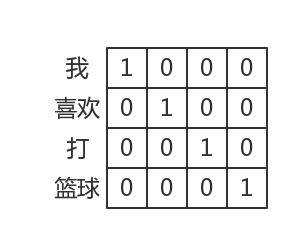
\includegraphics[scale=0.5]{picture/one-hot.png}
    \caption{One-hot表示法示意图}
    \label{one-hot}
\end{figure}

在这种转换方式下,针对具体语料可以快速得到每个单词的词向量,
程序能够容易地对文本进行处理计算,而且单词数据存储时也只需要保存一个
编号即可,节省了大量的存储空间。通过这种简洁的文本表示方式,传统自然语言处理
技术在许多任务中取得了很多令人满意的结果。

但本质上来说,One-hot表示方法就是给每个词语编号,然后以字典的方式来索引,这对于
形式复杂的单词来说实际上忽略了很多语义信息。在真实的语言中,
单词之间会存在多种不同的语义关系,例如同义词、反义词或一词多义等。而基于编码方式
表示单词的One-hot表示法生成的词向量全部正交(即词向量之间的余弦距离为0),
使得学习算法不能够从词向量中获取出这样的语义关系。
除此之外,当统计的文本足够多后,
One-hot表示法产生的向量会拥有一个巨大的维度,造成后续计算的维度灾难,
让后续学习算法的性能急剧下降,所以目前One-hot表示法已经很少被人使用。

(2)词的分布式表示法

从前面可以知道,传统的One-hot文本表示法形式过于简单,无法包含单词的
丰富语义,并且纬度往往过高,计算很不方便。为了解决这一问题,学者们开始尝试
将词语映射到低维的向量空间之中,以得到连续稠密的词向量,进而提出了
词的分布式表示方法。

词的分布式表示方法以Harris在1954年提出的分布假说\citing{firth1961papers}为理论核心,
认为具有相似语义环境的词语通常会表现出相同的语义,即一个词语的语义是由
该词语所处的上下文决定的。根据实现方式的不同,词的分布式表示方法
又大概可以分为基于矩阵与基于神经网络两种表示形式。

浅层语义分析(Latent Semantic Analysis,LSA)\citing{levy2015improving}
是基于矩阵的分布式表示法的
代表算法,该方法认为两个词如果多次出现在同一文档中,则这两个词在语义上具有相似性。
LSA使用词-文档矩阵(Occurences Matrix)来对文档进行描述,矩阵的一行代表一个单词,
一列代表一篇文档,矩阵中的每个元素则代表该词在文档中出现的次数,
并通过奇异值分解技术(Singular Value Decomposition,SVD)对矩阵进行降维,
去除矩阵中非必要的信息,最终得到文档的向量表示。

但是,这样的方法极度依赖语料库的统计信息,对于篇幅较长,内容较多的长文本
非常适用,但对于本文主要研究的短文本语料,由于单条文本长度很短,这类方法并不适合,
所以这里不做过多的讨论。

基于神经网络的词的分布式表示法通常也被称为词嵌入(Word Embedding),
一般以N-Gram语言模型为基础,利用神经网络的方式对文本进行建模。
N-Gram语言模型假定语言满足马尔科夫性,句子中的单词的出现与其前面出现的单词紧密相关,即第$n$个词的出现
只与前面$n-1$个词的出现相关,而和其他任何词都不相关。假设句子$S$由单词序列$\left (w_1,w_2,...,w_m  \right )$组成,
则N-Gram语言模型可表示为:
\begin{equation}
    \begin{aligned}
        P\left ( S \right )&=P\left ( w_1w_2...w_m \right )\\
        &=P\left ( w_1 \right )P\left ( w_2|w_1 \right )...
P\left ( w_i|w_{i-n+1}...w_{i-1} \right )...P\left ( w_m|w_{m-n+1}...w_{m-1} \right )
    \end{aligned}
    \label{n-gram}
\end{equation}
通过这样的实现方式,词嵌入方法能够充分对文本中复杂的上下文关系进行建模,同时还不依赖
语料库的统计信息,适用于各种类型的语料库。

\subsection{基于字的文本表示方法}
\label{char_rep}
基于字的文本表示方法是近几年刚刚兴起的一种文本表示方法,该方法与
基于词的文本表示方法相反,认为字才是文本的最小分割单元,并使用字向量序列
来表示文本。

基于字的文本表示方法最早被用于英文等字母语言,通过对26个字母进行类似One-hot表示法的编码操作,
将英文文本表示为连续的字母序列,
在文本分类、情感分析等任务中取得了不错的成果。
本质上来说,这种方法是利用英文是表音语言的特性,直接把毫无语义的字母序列输入
神经网络,利用其强大的学习能力,让网络自动学习文本的语义信息。

而对于中文这类的象形文字,由于汉字本身就包含非常丰富的语义且为数众多,
所以上述中的One-hot类表示方法并不适用。虽然国内学者这几年一直在
中文字向量领域不断研究,但没有关键性的突破,所以目前常见的中文字向量表示法
一般都是直接套用词向量模型,即把中文文本按字切分输入词向量模型进行训练。如何获得
性能优秀的中文字向量还没有一个通用的方法。

\section{词向量训练模型}
\subsection{神经网络语言模型}
神经网络语言模型(Neural Network Language Model,NNLM)是词向量模型中最经典的
模型,最早由Bengio提出\citing{bengio2003neural}。
该模型依照N-Gram语言模型的思想,
使用全连接的前馈神经网络(Feed Forward Neural Network,FFNN),
对语言进行建模,是N-Gram语言模型的一个完整实现,具体结构如图\ref{nnlm}所示。
\begin{figure}[h]
    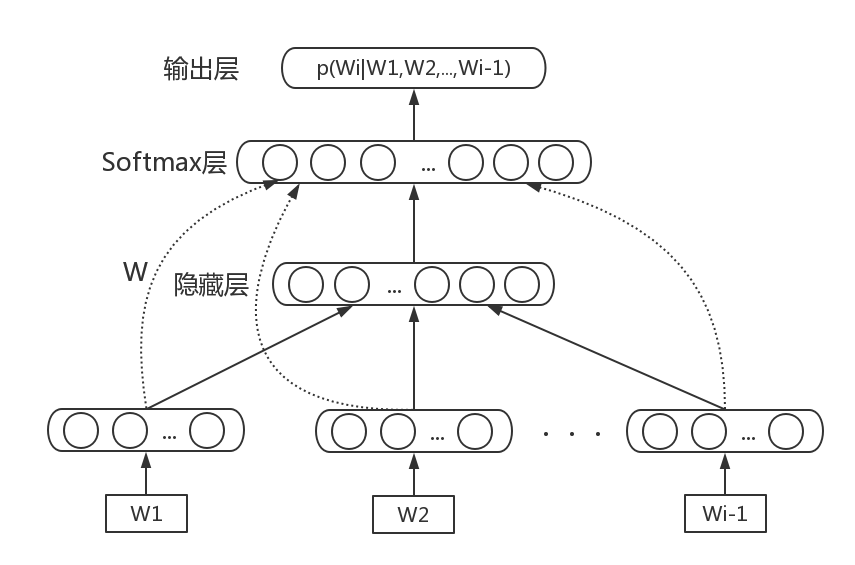
\includegraphics[scale=0.5]{picture/nnlm.png}
    \caption{神经网络语言模型}
    \label{nnlm}
\end{figure}

对于输入的单词序列$\left \{ w_{1},w_{2},...,w_{i-n+1} \right \}$
(目标词$w_i$的前$n$个单词),NNLM首先将它对应的单词向量拼接,得到上下文向量$h$,
如公式\ref{nnlm_input_eqn}所示。
\begin{equation}
    h = v_{w_1} \oplus v_{w_2} \oplus ... \oplus v_{w_{i-n+1}}
    \label{nnlm_input_eqn}
\end{equation}
然后将这个上下文向量$h$输入全连接的隐藏层进行非线性转换,得到中间向量$m$,
如公式\ref{nnlm_mid_eqn}所示。
\begin{equation}
    m = \tanh \left ( Hh+b_H \right )
    \label{nnlm_mid_eqn}
\end{equation}
这里$H$为隐藏层的权重矩阵,$b_H$则为对应的偏置矩阵。

隐藏层完成非线性转换后,将中间向量$m$输入后续的Softmax层。Softmax层
接收到$m$后首先会对其进行处理,然后利用Softmax函数得到最终的
条件概率,如公式\ref{nnlm_softmax_eqn1}与\ref{nnlm_softmax_eqn2}所示。
\begin{equation}
    s = Sm+b_S
    \label{nnlm_softmax_eqn1}
\end{equation}
\begin{equation}
    P\left ( w_i|w_{t-(n-1)},w_{t-(n-2)},...,w_{t-1} \right ) = 
    Softmax\left(s\right)=
    \frac{\exp s_i}{\sum_{k=1}^{|V|}\exp s_k}
    \label{nnlm_softmax_eqn2}
\end{equation}
其中,$S$与$b_S$是Softmax层的权重矩阵与偏置矩阵,
$V$表示语料库的统计词表,$|V|$则是词表中单词的数量,
$P\left ( w_i|w_{t-(n-1)},w_{t-(n-2)},...,w_{t-1} \right )$是模型
输出的条件概率,即在当前上下文条件下下一词为目标词$w_i$的概率。

最后对于训练语料库$D$,NNLM选用交叉熵损失函数作为模型的目标函数:
\begin{equation}
    L = -\sum_{w_t \in D}\log P\left ( w_t | w_{t-(n-1)},w_{t-(n-2)},...,w_{t-1} \right )
    \label{nnlm_loss_eqn}
\end{equation}


还有一点需要说的是,为了减少模型的训练时间,Bengio给模型添加了从输入层直接到Softmax层
的“捷径”,如图\ref{nnlm}中的虚线,此时Softmax函数的接收向量将由两个
输入组合而成,如公式所示。
\begin{equation}
    s = S\tanh \left ( Hh+b_H \right ) + Wh + b_S
\end{equation}

在文献\cite{bengio2003neural}中Bengio指出,添加该“捷径”可以在训练时减少
模型近一半的迭代次数,但也会降低词向量的质量,所以需要酌情使用该技巧。

总体来说,NNLM通过将输入层的词向量纳入训练参数的方式,让模型在能够在对语言进行建模
的同时得到单词的向量表示,可以说是一个里程碑式的模型,后续非常多的词向量训练模型
都是以它的思想为基本,在其之上改进与拓展。


\subsection{word2vec}
\label{sect_word2vec}
word2vec是Google公司于2013年发布\citing{mikolov2013distributed}的一款词向量构建工具。
该工具和NNLM一样,基于N元语言模型思想,通过神经网络对文本进行建模。
但不同的是,word2vec工具更加注重实用性与可操作性,内部对原始的NNLM删繁就简,
在保留核心结构的同时添加了多种加速技术,极大的提升了模型的使用效率。
在文献\cite{mikolov2013distributed}中作者Mikolov指出,在经过精心优化与
参数调整之后,word2vec工具在单机环境下一天24小时的训练量可以达到千亿级别。
而且虽然word2vec对NNLM做了很多删减,忽略了很多计算细节,但后续学者们的实验
都一致表明,word2vec生成的词向量在性能上并不劣于其他模型。

word2vec工具中包含有连续词袋模型(Continuous Bag-of-Words,CBOW)与
skip-gram两种模型,下面分别进行介绍:

(1)CBOW

CBOW的结构如图\ref{cbow}所示,可以看出,其核心架构与NNLM是类似的,
但很多实现细节上特别是训练方式都有非常大的不同。
\begin{figure}[h]
    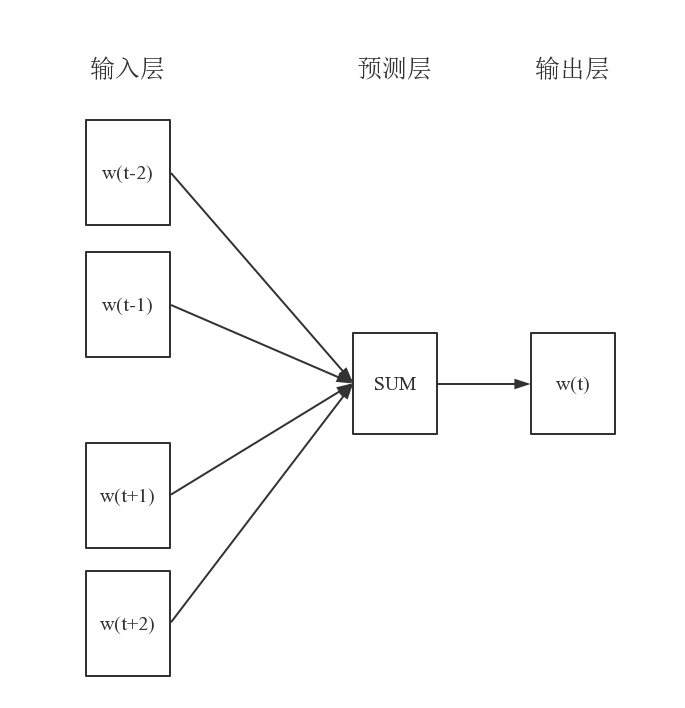
\includegraphics[scale=0.6]{picture/cbow.png}
    \caption{CBOW模型}
    \label{cbow}
\end{figure}

首先,CBOW以目标词前面和后面的$m$个单词共同作为目标词的上下文环境,而NNLM中只是以
目标词的前$n$个单词作为上下文。

其次,CBOW删除了NNLM中前向反馈神经网络的隐藏层,
将中间层直接和输出层的softmax节点连接,
并且忽略了目标词上下文的顺序信息,
把输入的全部词向量都汇聚在同一个隐藏层节点上(CBOW中称之为投影)直接得到上下文向量$c$
,如公式\ref{cbow_sum_eqn}所示。
\begin{equation}
    c = \frac{1}{2m}\sum_i w_{t+i}, j\in \{-m,...,m\}
    \label{cbow_sum_eqn}
\end{equation}

另一方面,CBOW为了优化NNLM中的全连接Softmax层,提供了两种加速技术
:层次Softmax技术(Hierarchical Softmax)与负采样技术(Negative Sampling)。

层次Softmax技术主要依靠Huffman Softmax树对原始Softmax函数近似求解,
以此简化计算。
模型训练时,CBOW首先依据整个训练语料中出现的单词建立Huffman Softmax树,
然后在预测时,让当前目标词的上下文向量从根节点出发,沿着Huffman Softmax树
不断向下进行二分类操作,直至叶节点,
最后将每次分类产生的概率进行乘积,就可以得到模型所需的条件概率$p(w_t|c)$。

通过这样的方式,对于包含$|D|$个不同单词的训练语料库$D$,
层次Softmax技术预测一个单词的时间复杂度只有$O\left ( \log|D| \right )$,
遍历整个训练语料的时间则是$|D|O\left ( \log|D| \right )$,
与NNLM中全连接Softmax的$O\left ( |D|^2 \right )$相比,有了非常大的提升。

负采样技术是CBOW提供的另一种加速计算技术,
该方法是噪声对比估计(Noise-Contrastive Estimation,NCE)的简化版本,
本质上是通过将目标词$w_t$替换为语料库$D$中的其他单词来构造一些称为
负样本的词串,以此将模型的优化目标变为最大化正样本的概率以及最小化负样本的概率。
对于语料库$D$,其目标函数如公式\ref{neg_loss_eqn}所示。
\begin{equation}
    L = \sum_{w\in D} \sum_{w\in \{w_t\} \cup w\in NEG\left ( w_t \right )} \log p\left ( w|C \right )
    \label{neg_loss_eqn}
\end{equation}
式中$C$表示$w_t$的上下文
(即$C=\{w_{t-n},w_{t-n+1},...,w_{t+n-1},w_{t+n}\}$),
$NEG(w_t)$表示目标词$w_t$的负样本集合,
条件概率$p\left ( w|C \right )$可以通过公式\ref{neg_p_eqn}得到。
\begin{equation}
    p\left ( w|C \right )=\sigma\left ( v_w\theta  \right )^{L(w)}+\left ( 1- \sigma\left ( v_w\theta  \right )\right )^{1-L\left ( w \right )}
    \label{neg_p_eqn}
\end{equation}
其中$v_w$为单词$w$的词向量,$L(w)$为标签函数,当$w$为正样本时$L(w)$取值为$1$,否则为$0$。

(2)Skip-gram模型

与CBOW模型相反,Skip-gram模型的思想是根据目标词预测与目标词相邻的单词,
模型结构如图\ref{skip-gram}所示。
\begin{figure}[h]
    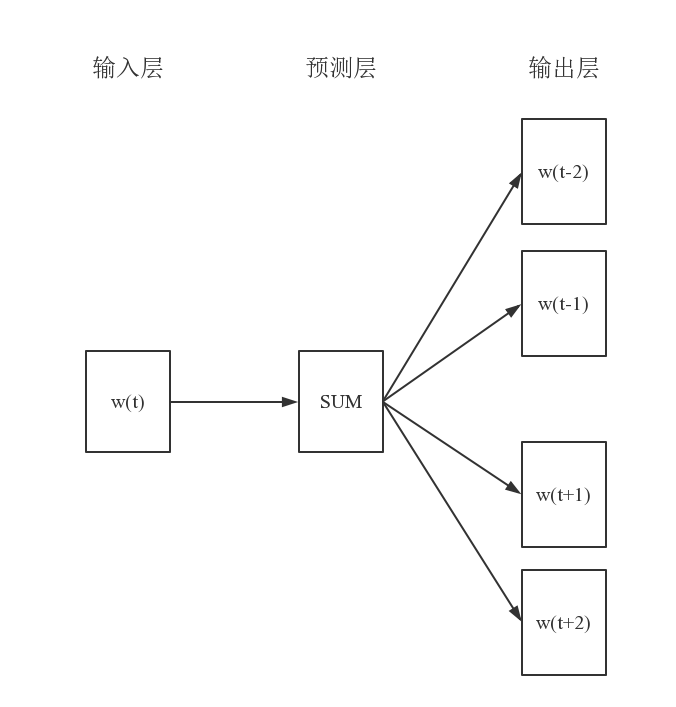
\includegraphics[scale=0.6]{picture/skip-gram.png}
    \caption{Skip-gram模型}
    \label{skip-gram}
\end{figure}
对于句子$S$,Skip-gram模型的目标函数如式\ref{skip-gram_eqn}所示。
\begin{equation}
    \arg \max_{\theta } \prod_{\left ( w,C \right )\in S}p\left ( c|w;\theta \right )
    \label{skip-gram_eqn}
\end{equation}
除此之外,Skip-gram模型的其他方面都与CBOW模型类似,这里不再赘述。


\section{基于神经网络的短文本分类方法}
与传统文本分类方法不同,基于神经网络的短文本分类方法使用更为复杂的
深度学习网络来提取文本特征,从而克服传统特征提取算法在短文本上的不足。
分类网络的一般框架如图\ref{classification_net}所示,
整体使用端到端训练(end-to-end training)\citing{chan2016listen}的方式
,以短文本的词向量矩阵作为输入数据,使用相应的特征提取网络从中提取语义特征,
得到文本特征向量,然后输入多类别分类器进行分类,最后与标注数据对比完成网络的训练。
本小结主要介绍两种常见的用于提取文本特征的深度学习网络。
\begin{figure}[h]
    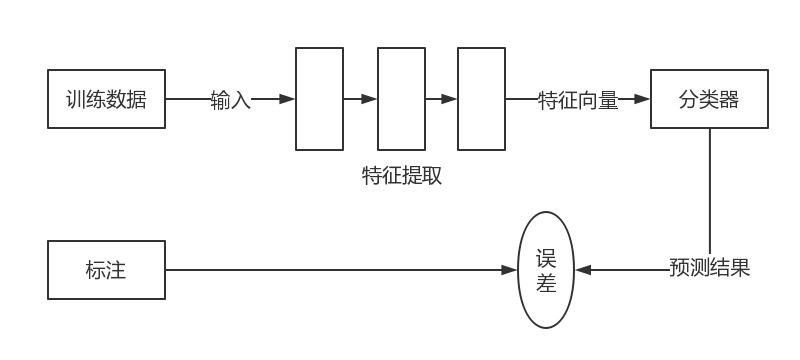
\includegraphics[scale=0.5]{picture/classification_net.png}
    \caption{短文本分类网络的一般结构}
    \label{classification_net}
\end{figure}

\subsection{卷积神经网络}
\label{cnn_section}
卷积神经网络(Convolutional Neural Network, CNN)\citing{lecun1989backpropagation}是一种前馈神经网络,
通过模仿猫脑皮层中用于局部感知和方向选择的神经元结构,有效降低了普通反馈神经网络的复杂性。

文本分类任务中,普通的神经网络模型通过构建一个全连接的网络对句子进行处理,
输入层的神经元直接接收文本的词向量,计算时隐藏层的某些节点会被输入的特征词激活(例如情感分类中“不”、“喜欢”等具有较强情感倾向的词),
从而得到有效的特征向量。但是在这样的网络结构中,单词之间的位置信息被忽略了,而同样的特征词,顺序与位置不同很可能导致不同的分类结构。
继续以情感分析为例,两个都包含“不”和“讨厌”这两个特征词的句子,“我不讨厌这部电影”表示的是好的情感,
而"我讨厌这部电影,不会买它的票"则表示坏的情感。

虽然可以通过n-gram等关注上下文的多元语言模型来解决这个问题,但在实际训练中,模型的窗口大小会成为一个非常大的问题。
窗口过小会使得模型效果不佳,窗口过大则导致计算量爆炸。并且,相似的单词在模型中不能共享参数、权重,
相似单词无法获得交互信息,这也会增加模型的计算量。

经过一系列探索,学者们发现卷积神经网络能够有效解决上述问题:
基于局部感知野理论,一个隐藏层神经元只与部分词语连接,可以达到类似多元语言模型的
效果,学习到更多的文本特征,并且在特征的识别与学习时只关注词语的相对位置,忽略它们的绝对位置,
也加速了学习过程;基于参数共享理论,相似特征使用同样的参数来提取,极大的降低了
网络模型的总体参数数量,加快了模型的训练。



卷积神经网络由三层网络组成:卷积层、池化层、光栅层,整体结构如图\ref{Text_CNN}所示。
\begin{figure}[h]
    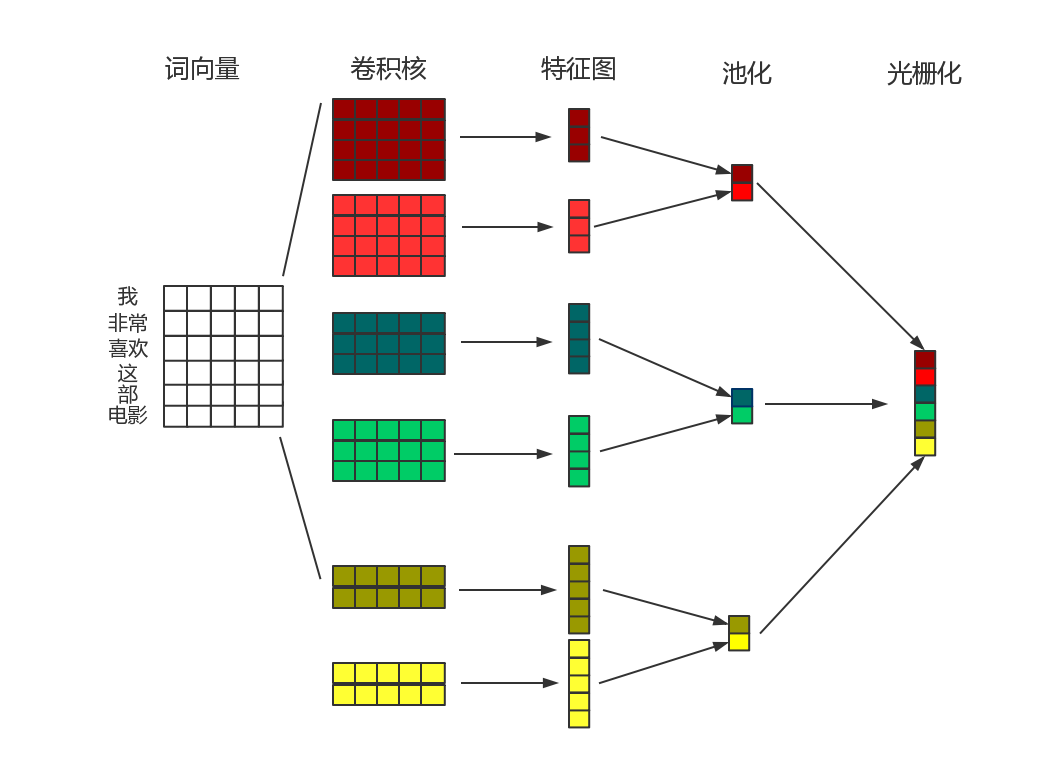
\includegraphics[scale=0.4]{picture/Text_CNN.png}
    \caption{卷积神经网络结构}
    \label{Text_CNN}
\end{figure}

(1)卷积层

卷积层主要用于特征提取,通过多个卷积核,对输入数据进行卷积计算,最后得到相应的特征图(Feature Map)。

卷积计算是通信领域中常见的计算方法,假设有二维离散函数$f\left ( x,y \right )$和$g\left ( x,y \right )$,
那么它们的卷积定义如公式\ref{cov_eqn}所示。
\begin{equation}
    f\left ( x,y \right )\ast g\left ( x,y \right )=\sum_{u}^{\infty }\sum_{v}^{\infty }f\left ( u,v \right )
g\left ( x-u,y-v \right )
    \label{cov_eqn}
\end{equation}

卷积核是提取特征的主要工具,相当于图像处理领域中的滤波器,
可以从输入数据中提取一类特征,其他类特征则需要另外的卷积核来提取,所以
卷积层通常包含有多个卷积核。一个卷积核包含参数矩阵$W$和偏置项$b$,计算过程如公式\ref{cov_layer_eqn}所示。
\begin{equation}
    h=f\left ( W\ast x+b \right )
    \label{cov_layer_eqn}
\end{equation}
其中$h$表示产生的特征图,$f$是激活函数。

具体到文本分类任务,输入数据为文本的词向量,
卷积核通常覆盖上下几行单词,并且宽度与词向量宽度相同(如图中卷积核部分所示),
这样就能够捕捉到多个连续词之间的语义特征,并且能够在同一类特征计算时共享参数。

(2)池化层(Pooling layer)

卷积层输出的特征图在数据纬度上与原始输入数据相比并没有减少很多,并且由于
存在多个卷积核,实际上输出数据往往会增多,如果不做处理,无疑会增加网络的复杂度,
产生巨大的计算量。

池化层也称为下采样层,在卷积层之后,对特征图进行降维操作(即池化操作)。
常见的池化操作有最大池化、最小池化和平均池化。其中最大池化是现在最常见的池化方式,
该方法将特征图分为多个子块,每个子块内部取最大的一个数据输出,
从而达到降低特征图纬度的目的。

对于文本数据,池化操作可以将长度不同的句子转化为长度相同的特征向量,方便后续统一处理。
另外最大池化还能够保留显著的特征。卷积核提取特征时,每一种卷积核会专注检测某一种含义的
词组,如果这种类型的词组出现了,该卷积核此时的输出值就会非常大,
通过最大池化就能够尽可能的将这些信息保留,同时忽略其他无关的信息。

(3)光栅层

输入数据经过卷积层与池化层计算之后,得到的是一系列特征图,而卷积神经网络之后的结构接收的
输入可能是一个特征向量。因此需要将这些特征图中的数据依次取出,排列成一个向量,
如网络结构图\ref{Text_CNN}中的光栅化部分所示。


\subsection{循环神经网络}
\label{rnn_section}
循环神经网络(Recurrent Neural Network,RNN)也叫做递归神经网络,是深度学习中另一个重要的网络模型。
RNN的结构如图\ref{RNN}所示,其特点是隐藏层节点不仅接收输入层的数据,还会接收上一个节点的输出数据作为另一个输入源,
这让RNN可以非常自然的处理序列数据,如文本、语音、视频等。
\begin{figure}[h]
    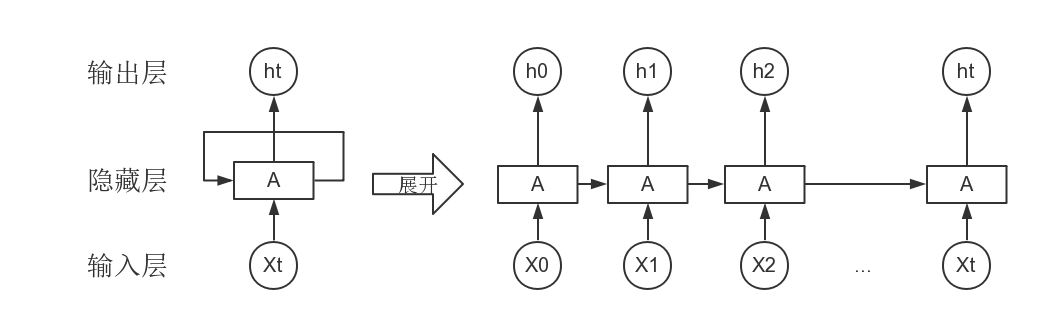
\includegraphics[scale=0.4]{picture/RNN.png}
    \caption{循环神经网络结构}
    \label{RNN}
\end{figure}
RNN中隐藏层节点包含三个部分,输入参数矩阵$U$、记忆参数矩阵$W$以及输出矩阵$V$,
对于节点$t$,计算公式如\ref{rnn_hidden_eqn}所示。
\begin{equation}
    s_t=f\left ( Ws_{t-1}+Ux_t \right )
    \label{rnn_hidden_eqn}
\end{equation}
其中$s_t$为中间向量,同时送往下一个隐藏层节点$t+1$与输出节点$h_t$,$f$一般为非线性激活函数
,$s_{t-1}$是上一个节点输出的中间向量。

对于文本分类任务,由于隐藏层中最后一个隐藏节点能够接收到之前所有节点的输出信息,
所以通常将该节点的输出向量作为网络最后生成的文本特征向量。

RNN模型的优点是对文本这类顺序数据有优秀的建模能力,能够突破n-gram模型中窗口大小的限制,
提取长间隔的单词之间的特征,
隐藏层最后一个节点的输出甚至可以包含前面所以单词的特征信息。
同时模型长度可变,对任意长度的文本都可以直接处理。

RNN模型的缺点也十分明显,那就是模型训练十分困难。根据反向传播算法,
RNN模型训练时会将梯度在隐藏层之间以乘积的形式传播,如果梯度大于$1$,
则多次相乘会使其指数级上升,引起梯度爆炸(Gradient Exploding);相反如果小于$1$,都次相乘后梯度逐渐为$0$,
又引起梯度消失(Gradient Vanishing)。

长短期记忆网络(Long Short Term Memory networks,LSTM)
\citing{hochreiter1997long}是对传统RNN模型的改进,
它将每个隐藏层节点看做“记忆细胞”,
在里面增加一种称为“门”的结构,对输入输出数据加以控制,从而有效解决梯度爆炸与梯度消失的问题。

LSTM的结构如图\ref{LSTM}所示,每个节点包含三个门结构(图中$\sigma $部分),
分别为遗忘门(Forget Gate)、输入门(Input Gate)与输出门(Output Gate)。
每个门由一个$Sigmoid$神经网络层和一个相乘操作组成,其中$Sigmoid$层输出$0\sim1$之间的值,
表示对应的部分信息是否应该通过,并利用相乘操作作用在输入或输出信息上,$0$值表示不允许信息通过,
$1$值表示让所有信息通过。
\begin{figure}[h]
    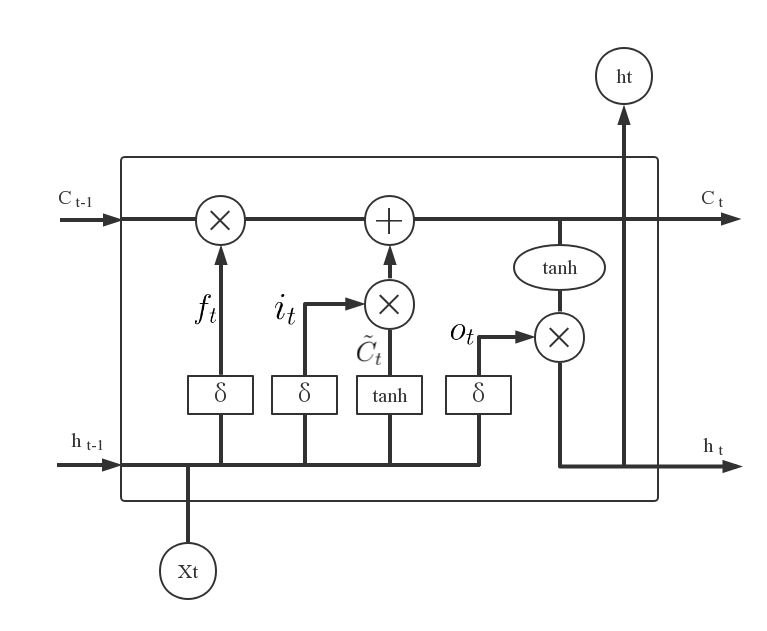
\includegraphics[scale=0.5]{picture/LSTM.png}
    \caption{长短期记忆网络}
    \label{LSTM}
\end{figure}

在一次计算过程中,LSTM节点首先计算遗忘门,公式如\ref{forget_gate_eqn}所示。
\begin{equation}
    f_t=\sigma\left ( W_f \cdot [h_{t-1},x_t]+b_f \right )
    \label{forget_gate_eqn}
\end{equation}

其中$W_f$与$x_t$是遗忘门中$Sigmoid$层的参数矩阵和偏置矩阵,$f_t$为遗忘向量,
里面的每一位都对应$C_{t-1}$中的一个数据,用来控制信息的流入。

第二步是将输入数据$x_t$存储到节点中,并更新节点状态。
这一步首先计算第二个门结构——输入门的$Sigmoid$层与一个tanh层,
得到两个候选值$i_t$与$\tilde{C}_t$,如公式\ref{input_gate_eqn}与\ref{input_gate_eqn2}所示。
\begin{equation}
    i_t=\sigma\left ( W_i \cdot [h_{t-1},x_t]+b_i \right )
    \label{input_gate_eqn}
\end{equation}
\begin{equation}
    \tilde{C}_t=\tanh\left ( W_C \cdot [h_{t-1},x_t]+b_C \right )
    \label{input_gate_eqn2}
\end{equation}

然后根据公式\ref{input_gate_eqn3}得到节点的新状态$C_t$。
\begin{equation}
    C_t=f_t \ast C_{t-1} + i_t \ast \tilde{C}_t 
    \label{input_gate_eqn3}
\end{equation}

最后,节点通过第三个门结构——输出门,得到输出向量,如公式\ref{output_gate_eqn}所示。
\begin{equation}
    \begin{split}
        o_t&=\sigma\left ( W_o \cdot [h_{t-1},x_t]+b_o \right ) \\
        h_t &= o_t \ast \tanh\left ( C_t \right )
    \end{split}
    \label{output_gate_eqn}
\end{equation}

通过增加门结构,LSTM有效避免了传统RNN在训练上的问题,但与CNN相比,
其训练效率依然十分低下,实际使用中常常造成问题。
因此,本文对短文分类算法的优化,将融合RNN与CNN,结合它们的优点,构建一个
对于中文短文快速有效的分类模型。

\section{Attention Model}
Attention Model是近几年兴起的一个新型模型,在很多场景被证明有效。
模型以认知心理学中的人脑注意力理论为核心,认为人脑在处理具体任务时,对于相关事物的注意力会集中在
某一个特定的地方,忽略其他无关的地方,而不是对每个地点分配相同的注意力。
通过这样的理论,Attention Model
能够合理的分配模型的计算资源,并且还可以避免非关键数据对结果的影响。
Attention Model最先被应用与计算机视觉领域中
的图片识别等问题,取得了很好的成果,随后在自然语言处理领域也获得了优秀的成绩。
\iffalse
下面将以编码-解码模型中的Attention机制为例,
说明Attention Model的基本知识。

编码-解码模型是自然语言处理领域中一个非常普遍的模型,它通过编码器将输入向量编码为中间
变量,再用解码器解码成输出向量,完成输入数据到另一组输出数据的转变,
从而实现多种内容转换任务,如机器翻译、文本复述等。
同时编码-解码模型的编码器与解码器没有具体限定,可以使用
各种各样的深度学习模型,如CNN、RNN等,这让模型具有很强的泛用性,能够适合各种应用场景。
编码-解码模型的一般架构如图\ref{Encoder}所示。
\begin{figure}[h]
    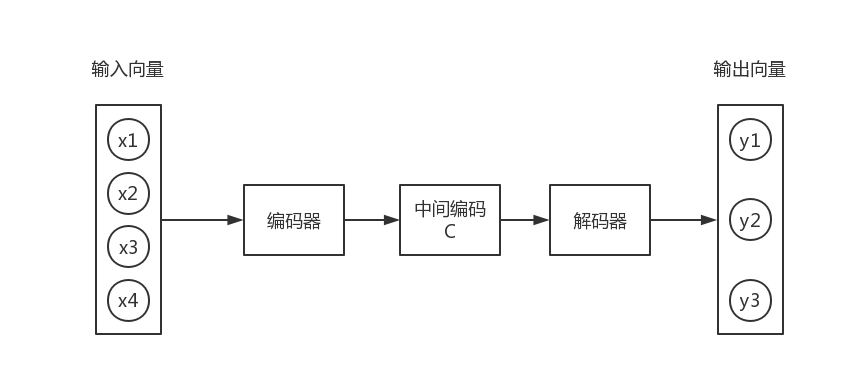
\includegraphics[scale=0.5]{picture/Encoder.png}
    \caption{编码-解码模型架构图}
    \label{Encoder}
\end{figure}
\fi

例如,对于编码-解码模型,输入数据一般是一个长度为$n$向量序列$X$($X= \left \{x_1,x_2,x_3,...,x_n \right \}$),
输出则是一个长度为$m$的向量序列$Y$($Y= \left \{y_1,y_2,y_3,...,y_m \right \}$)。
模型运行时,编码器根据一定的映射规则对输入序列进行编码,得到中间编码$C$,表达公式如\ref{encode_eqn}所示。
\begin{equation}
    C=Encode\left ( x_1,x_2,x_3,...x_n \right )
    \label{encode_eqn}
\end{equation}
之后解码器对中间编码$C$进行解码,得到输出序列$Y$,计算公式如\ref{decode_eqn}所示。
\begin{equation}
    y_i=Decode\left ( C,y_1,y_2,y_3,...,y_{i-1} \right ),i=1,2,3,...,m
    \label{decode_eqn}
\end{equation}

可以看出解码器在计算输出序列$Y$时,对于每一个输出子项$y_i$用到的数据信息是一样的,都是
输入序列$X$编码后得到的中间编码$C$,
即输入序列$X$对输出序列$Y$中每一个子项的影响是相同的。这样的方式无疑忽略了
很多细节,在一些任务中甚至直接影响了输出结果。比如机器翻译任务,
一个词的翻译虽然与上下文和词本身同时有关,但对于人名机构名等名词,
翻译时词本身的影响必定较重,而其他的动词形容词等则可能上下文的影响较大,所以简单
输入序列同比例的作用在输出序列之上并不是一个好的方法。

而加入Attention Model之后,
编码器的输出不再是一个完整的中间编码$C$,而是输入序列$X$在编码阶段的历史状态$C_i$,
如公式\ref{attention_encode_eqn}所示。
\begin{equation}
    C_i=\sum_{j=1}^{n}\alpha_{ij}Encode\left ( x_j \right )
    \label{attention_encode_eqn}
\end{equation}
其中$\alpha_{ij}$表示当前输入子项$x_j$的注意力权重,这个值越高,表明$x_j$对结果
越重要。

解码器根据历史状态$C_i$得到优化后的输出序列,如公式\ref{attention_decode_eqn}所示。
\begin{equation}
    y_i=Decode\left ( C_i,y_1,y_2,y_3,...y_{i-1} \right ),i=1,2,3,...,m
    \label{attention_decode_eqn}
\end{equation}

总体来说,Attention Model本质上就是在模型的输出结果上添加一个注意力权重,
筛选对结果重要的数据项,同时过滤对结果影响较低的数据项,以此优化模型的输出效果。
这一思想在短文本分类任务中同样适用,因为对于短文本文本分类任务,确定分类结果的
往往是文本的几个关键词,如情感分析中的“喜欢”、“讨厌”等词,如果能够判断出这些关键词,
就可以极大的增强分类模型的结果。

\section{本章小结}
本章首先对文本表示的两种方法进行了介绍,
接着引出了基于神经网络的短文本分类方法,并阐述了
卷积神经网络和循环神经网络在文本分类任务中的应用。
这些基础内容为本文的后续工作提供了坚实的理论基础,后续章节将根据这些知识
搭建一个中文短文本分类模型。
\end{document}
    \chapter{中文文本表示方法的研究和改进}
文本的向量化表示是中文短文本分类研究的核心之一。传统的One-hot表示法虽然简单快速,
但忽略的太多的语义信息,在实际使用中效果较差,达不到人们的预期。
词嵌入技术将文本中的单词映射到一个连续的向量空间之中,
让意思相近的单词能够在向量空间中彼此靠近,
这让深度学习模型能够直接通过文本向量获取相关的语义信息,
更有利与进一步的文本分类工作。因此,本章节将根据汉字的特点,充分利用汉字中蕴含的丰富信息,
设计一种新颖的适合中文的词向量模型。

本章节首先介绍汉字中部首的一些特性,然后简要概述现阶段中文文本表示的一些方法,
再详细介绍本文设计的基于部首信息的词向量与字向量模型,最后根据实验结果论述模型的有效性。
\section{汉字偏旁部首的语义信息}
\label{radical_information}
汉字是四大古老文字之一,传说起源于黄帝的史官仓颉。根据内在结构的不同,
汉字可分为独体字和合体字。独体字源于最早的甲骨文,是象形文字的延续。
如图\ref{char_fish}所示,每一个独体字都可以看做是现实事物的抽象,本身不可分割,整体表达一个语义。
合体字则是在独体字之上发展而来的。汉字系统初期几乎都为独体字,数量相对较少,
大量事物以通假字来表示,使文字表述存在较大歧义。为了能更精确的表述,
人们以基本的象形独体字为基础,通过组合的方式构造大量新的文字。
比如最早海上的交通工具就只有:“舟”一种,但演化到现在,
细分成“舨、舟、艇、船、舰”等不同小大规模与形制的“舟”。
到了现代,合体字成为了汉字的主体,占90\%以上。
\begin{figure}[h]
    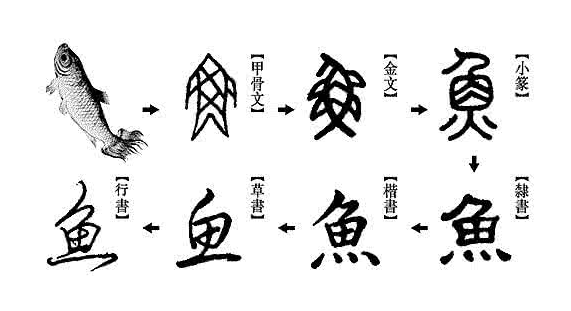
\includegraphics[scale=0.6]{picture/char.png}
    \caption{鱼字的演化过程}
    \label{char_fish}
\end{figure}

部首是构建合体字的主要单元。这一概念最早由公元2世纪汉朝的许慎提出,
他在其著作《说文解字》中将合体字中重复出现的部分加以归类,分成540个“部”。
“部”之后发展为现在的部首,
现在通用的部首由清朝康熙五十五年(1716年)成书的《康熙字典》所制定,共214个。

汉字的部首通常由某一个独体字演化而来,而且与英语等字母语言不同的是,
部首是汉字语义的重要组成部分。很多时候,
部首能够让我们在没有任何上下文的情况下大致理解或推测一个汉字的意义。
这也就是说,在学习汉字语义表示的时候,部首所固有的语义特征能够提供额外的信息。
举例来说,通过由“人”字演变而来的部首“亻”,我们可以很清楚的知道“你”、“他”、“伙”、
“侣”、“们”等字全部都和人有关。并且这种根据部首获得的语义信息与N-gram模型这类基于相邻$N$
个单词获得的信息本质上是不同的。因此在词向量模型中添加部首的语义特征能够
给每个词语增加丰富的语义信息,提升中文词向量的质量。

偏旁是构建合体字的另外一个重要单元。虽然在合体字特别是形声字中,
偏旁往往表示事物的读音,但是对于会意字与部分形式字,偏旁任然含有可利用的语义信息。
比如汉字“武”,它的部首为“止”,是“趾”的本字,表示脚,偏旁为“戈”,表示武器,
整体表示人拿着武器行走;对于汉字“茱”,部首的“艹”表示植物,偏旁“朱”则表示红色,兼
表示字音。所以只要善加利用,偏旁也能够为词向量的构建提供很多语义特征。

\section{中文文本表示方法}
中文文本的词向量构建方法一直是中文自然语言处理领域的焦点。
在研究初期,研究者们尝试直接使用英文词向量工具
(如\ref{sect_word2vec}中介绍的CBOW模型和Skip-gram模型)
在经过分词之后的中文语料上训练词向量。
但是这种做法很明显存在问题:大多数英文词向量工具在训练时都将词作为最小的操作单位,
而忽略了词语内在的一些形态信息(morphological information)。和英语等字母文字不同,
中文词语之中的汉字任然含有丰富的语义信息。比如“智能”这个词,
它的语义信息一方面我们可以从语料中相关的上下文学习,就像word2vec模型一样。
另一方面我们也可以根据组成这个词的两个汉字“智”和“能”推测出来(“智”为智慧,“能”为能力)。

为了解决上述问题,充分利用中文词语的语义信息,陈志勇等人\citing{chen2015joint}在
普通CBOW模型上加入汉字信息,提出了CWE模型。随后Xu等人\citing{xu2016improve}在
CWE模型的基础上,赋予词中每个字权重,优化整个词向量模型。
但这些模型都没有利用汉字中的偏旁部首,忽略了所有文字内部的信息。

另一方面,Sun等人\citing{sun2014radical}在CBOW模型的基础上增加了部首信息来训练中文字向量;
Yu等人\citing{yu2017joint}在CWE模型中结合“部首-汉字”与“汉字-词”的信息,
设计了一个多粒度的词向量模型。但这些方法都只是简单的在模型中添加了部首信息,没有考虑
到部首的演化,即没有将部首与意义对应的汉字联系起来(比如“氵”-“水”),
这使得模型从部首获得的信息非常有限,影响生成的词向量的质量。


\section{部首信息增强的中文词向量构建方法}
根据上一小节中介绍的其他学者在中文词向量模型上的种种成果以及汉字中偏旁部首的特性,
本文设计了一种新的中文词向量模型——部首信息增强的中文词向量模型(Radical Enhanced Chinese Word Embedding Model,RECWE)。
RECWE以word2vec工具的CBOW模型为基础,在模型的预测层中增加一个代表“偏旁部首-汉字”信息的隐藏层,
增强每个词的语义信息。同时,RECWE将输入文本从简体转换为繁体,并对每个字的部首进行语义转换,
最大程度上丰富输入词语的语义信息。
\subsection{文本预处理}
由于实验所用的语料大多来自于互联网,其格式编码往往没有统一,所以需要首先进行相关处理,得到
一个相对整齐一致的文本数据。同时为了让词向量模型能够获取部首信息,还需要进行语义相关的一些
处理。整体的预处理流程包括:

(1)特殊字符过滤

网络搜集的数据常常是用户随意产生的非规范文本,里面会包含大量和文本语义无关的特殊字符与
标点符号,因此需要对这些符号进行过滤,只保留文本以及相关英文专有名词。

(2)全半角转换

由于使用的语料来源广泛,相互之间没有共同的格式规范,文本中的数字、英文字母等同时存在全角
和半角的格式,为了让之后的分词工作能够准确快速,需要将所有数字及字母统一转换为半角字符。

(3)分词

本文所使用的分词工具为java语言实现的Ansj中文分词开源库。该库基于n-Gram、CRF与HMM
算法,分词速度达到每秒钟大约200万字左右,准确率能达到96\%以上,并且实现了
中文分词、中文姓名识别、用户自定义词典、关键字提取、自动摘要、关键字标记等重要功能,
对于短文本语料有较好的表现。

(3)繁简转换

新中国成立后进行了一系列汉字简化工作,现阶段中国大陆地区使用的简体汉字是1956年发布的\citing{su2007hanzi}。
但在汉字简化工作中,存在一些不适当的简化,使得简化字的部首与原始繁体字的部首不同,
出现汉字语义上的偏差。例如繁体字中的“羆”字,分解后的偏旁部首为“罒”和“熊”,
意指一种很大的熊,可是简化后却变为了“罴”,相应的偏旁部首为“罢”和“灬”,失去了原来的含义。
而且简化工作还将多个繁体字归并为一个简体字,即“一简对多繁”,这就造成了理解上的困难和歧义,并生成了一批多音字,让简体词语中的字不能
很好的反应这个词的语义,增加了词向量模型学习词语语义的难度。比如繁体的词语“干(gān)涉”、“乾(gān)燥”、“幹(gàn)部”中的“干”、“乾”和“幹”,简化后统一变为
“干”字,让模型很难区分。

因此,为了更好的表达原始语料中文本的语义,让模型能够正确捕获中文词语中的部首的语义信息,
需要将原本的简体文本全部转换为繁体文本。本文使用汉语言处理包HanLP作为繁简转换工具,
该处理包能够有效区分同一个简体字对应的多个繁体字,并且可以识别简繁分歧词,
如“打印机”与“印表機”。

(4)部首提取与语义转换

为了让RECWE模型能够直接获取汉字的部首信息,预处理阶段会将词语中的汉字拆解为
对应的偏旁部首。但是,根据\ref{radical_information}节中关于部首的介绍,
由某一个独体字演化而来的部首,
在合体字中会为了书写美观往往需要进行一定的拉伸或收缩,
来适应合体字整体的字型。例如“水”字在合体字中拉伸成了部首“氵”,
“食”字在合体中收缩为了部首“飠”。
因此本文提取了常见字的部首并构建了一个转换表(如表\ref{char_tran_form}所示),
将部首转换为对应的独体字,从而让RECWE模型能够有效识别出这种内在联系,
比如“木”字与“案”、“板”、“森”、“李”等字,“水”字与“泉”、“河”、“海”等字。

\begin{table}[h]
\caption{常见部首转换表}
\begin{tabular}{|c|c|c|c|}
    \hline
    部首 & 对应汉字 & 部首 & 对应汉字 \\
    \hline
    艹 & 艸 & 亻 & 人\\
    \hline
    刂 & 刀 & 犭 & 犬\\
    \hline
    灬 & 火 & 釒 & 金\\
    \hline
    麥 & 麥 & 飠 & 食\\
    \hline
    礻 & 示 & 月 & 肉\\
    \hline
    攵 & 攴 & 罒 & 网\\
    \hline
    扌 & 手 & 氵 & 水\\
    \hline
    糹 & 糸 & 耂 & 老\\
    \hline
    牜 & 牛 & 忄 & 心\\
    \hline
    衤 & 衣 & 王 & 玉\\
    \hline
    辶 & 走 & 疒 & 病\\
    \hline
\end{tabular}
\label{char_tran_form}
\end{table}
\subsection{部首信息增强的中文词向量模型}
本文提出的RECWE模型结合了中文的单词、汉字以及偏旁部首的语义信息,旨在构建适合中文的高效词向量。
RECWE模型基于CBOW模型\citing{mikolov2013distributed},
通过词的平均上下文向量和字与部首的平均上下文向量预测目标词,
并且使用这两个上下文向量的预测损失的和作为目标函数。

RECWE模型结构如图\ref{RECWE}所示,其中$w_i$表示需要预测的目标词,$w_{i-1}$和$w_{i+1}$
分别表示文本中目标词$w_i$左边和右边的词。$c_{i-1}$和$c_{i+1}$表示$w_{i-1}$和$w_{i+1}$中的汉字,
$r_{i-1}$和$r_{i+1}$则分别表示$c_{i-1}$和$c_{i+1}$对应的部首(经过表\ref{char_tran_form}转换),
$s_{i-1}$和$s_{i+1}$表示$c_{i-1}$和$c_{i+1}$的偏旁。
通过在预测层将两个上下文向量并列以及共享隐藏层参数,字向量与偏旁部首向量在训练时能够很好的
影响词向量,从而让最终训练得到的词向量能够充分反映出词语内部汉字与部首的语义信息。
\begin{figure}[h]
    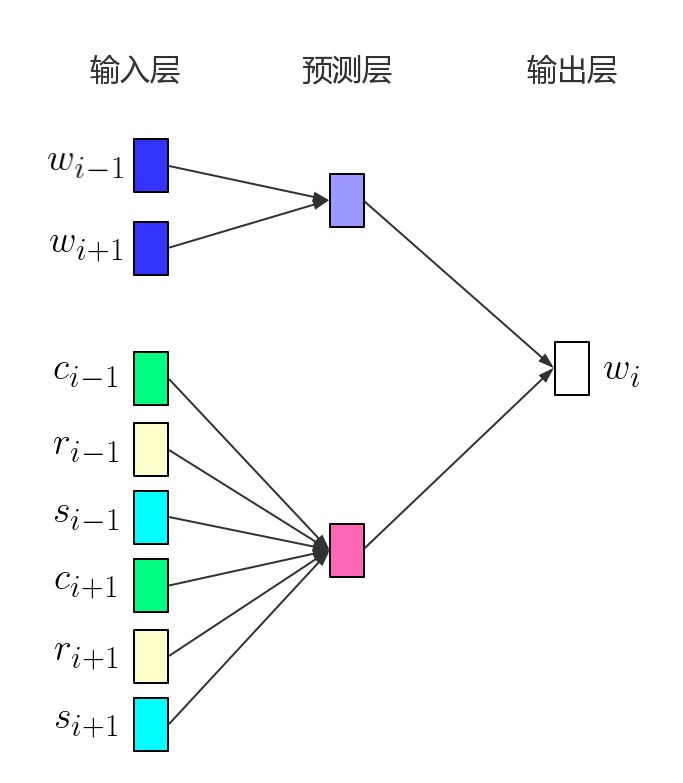
\includegraphics[scale=0.4]{picture/RECWE.png}
    \caption{RECEW模型结构}
    \label{RECWE}
\end{figure}

与CBOW模型类似的,RECWE模型的目标函数是两个上下文向量对于目标词$w_i$的条件概率的对数似然函数,
如公式\ref{RECWE_target_fun}所示。
\begin{equation}
    L\left ( w_i \right )= \sum_{k}^{2}\log P\left ( w_i | h_{i_k} \right )
    \label{RECWE_target_fun}
\end{equation}
其中$h_{i_1}$和$h_{i_2}$分别表示词的上下文向量和字与部首的上下文向量。
通过这样

每个上下文向量对于目标词$w_i$的条件概率$p\left( w_i|h_{i_k}\right )$可以利用softmax函数求解,
如公式\ref{conditional_pro_fun}所示。
\begin{equation}
    p\left ( w_i | h_{i_k} \right )=\frac{\exp \left ( h_{i_k}^{T}\hat{v}_{w_i} \right )}{\sum_{j=1}^{N}\exp \left ( h_{i_k}^{T}\hat{v}_{w_j} \right )},k=1,2
    \label{conditional_pro_fun}
\end{equation}
其中$\hat{v}_{w_i}$表示目标词$w_i$的“输出”向量,$\hat{v}_{w_j}$表示输入语料中每个词的“输出”向量,
$N$表示输入语料的长度。

上下文向量$h_{i_1}$是上下文窗口中每个词的“输入”向量的平均值,通过式\ref{word_context_fun}得到:
\begin{equation}
    h_{i_1}=\frac{1}{2T}\sum_{-T\leq j\leq T,j\neq 0}v_{w_{i+j}}
    \label{word_context_fun}
\end{equation}
式中的$T$表示上下文窗口的大小,$v_{w_{i+j}}$是上下文窗口中单词的“输入”向量。

类似的,字与部首的上下文向量$h_{i_2}$是上下文窗口中每个词对应的字及其偏旁部首的“输入”向量的平均值,计算公式如\ref{char_context_fun}所示。
\begin{equation}
    h_{i_2}=\frac{1}{X}\sum_{-T\leq j\leq T,j\neq 0} v_{c_{i+j}}+v_{r_{i+j}}
    \label{char_context_fun}
\end{equation}
其中$v_{c_{i+j}}$和$v_{r_{i+j}}$分别表示字和偏旁部首的“输入”向量,$X$为
$v_{c_{i+j}}$和$v_{r_{i+j}}$的数量。

于是,对于语料库$D$,RECWE模型的整体对数似然函数如公式\ref{overall_target_fun}所示。
\begin{equation}
    L\left ( D \right )=\sum_{w_i \in D}L\left ( w_i \right )
    \label{overall_target_fun}
\end{equation}

RECWE模型的训练算法采用CBOW模型实现的负采样(Negative Sampling,NEG)算法\citing{mikolov2013distributed},
该算法是NCE(Noise Contrastive Estimation,NCE)算法的一个简化版本,
其中心思想是将当前窗口内的词语分为正样本(需要预测的目标词)及负样本(目标词之外的其他词),
然后加权随机选取负样本进行更新,每个负样本的权重与其在语料库中出现的次数成正比,
以此来提高模型的训练速度并改善所得词向量的质量。
结合随机梯度上升技术,
基于负采样的RECWE模型能够快速获得中文词向量。



%添加点
%可以添加负采样的介绍

\section{部首信息增强的中文字向量构建方法}
\subsection{中文字向量概述}
中文分词技术虽然已相对成熟,但准确率任然达不到100\%,分词结果依然存在一定的错误。
对于本文主要研究的中文短文本,由于其大多来自与用户在互联网的互动,如腾讯空间说说、新浪微博、
淘宝商品评价等,相比于长文本具有很强的随意性,充斥着大量的口语化表达方式,
有些句子甚至存在语病,这更进一步增加了分词的难度,使得分词结果很不理想。
而错误的分词结果会极大影响后续的词向量模型,降低词向量的质量。

字向量是解决分词问题的一个方向,
来源于英文文本处理中字符级别(Character-level)的文本表示方式
\citing{zhang2015character}。
国内学者通过给汉字编码\citing{chen2015joint, 胡浩2017汉字固有属性},或将汉字转换为汉语拼音\citing{zhang2015character},
将文本表示为连续的向量,从而绕过分词的步骤,然后通过循环神经网络等深度学习技术直接从
字向量中学习文本特征,取得了不错的成果。但这些方法得到字向量类似于One-hot向量,
没有反应出每个字直接语义上的联系,忽略了大量的语义信息。
因此,作为RECWE词向量模型的补充,本文设计了一个能够利用汉字部首信息的字向量模型,
为后续的分类模型提供更多的文本信息,克服分词错误带来的影响,最终提升分类准确率。


\subsection{部首信息增强的中文字向量模型}
\section{实验及其结果分析}
    \chapter{Attention-Based字词结合卷积循环中文短文本分类模型}
\label{4_section}
短文本分类技术在自然语言处理领域中扮演着重要的角色,
在垃圾信息过滤、语义分析、自动问答等任务中有着广泛的应用。
本节主要介绍了本文实现的卷积循环特征提取网络以及根据该特征提取网络建立的
Attention-Based字词结合中文短文本分类分类模型。
在进行分类任务时,
特征提取网络由于结合了基于局部感知域理论设计的卷积神经网络以及基于时间记忆理论设计的循环神经网络,
能够有效地提取丰富全面的文本特征。
同时模型引入了注意力机制,可以进一步优化提取出的文本特征向量,防止特征向量信息冗余或信息缺失。
而采用双通道结构的分类模型,同时解析词向量与字向量数据,极大的丰富了原始语料的语义信息,
提升了网络的准确率。本文设计的中文短文本分类网络有以下几个新特点:
\begin{enumerate}
    \item 使用优化的卷积循环神经网络
    \item 引入了注意力机制优化文本特征向量
    \item 使用双通道结构同时处理字向量数据与词向量数据
\end{enumerate}

\section{卷积循环神经特征提取网络}
\label{CLSTM_section}
根据\ref{cnn_section}小节与\ref{rnn_section}小节的介绍,我们知道
卷积神经网络和循环神经网络在特征提取方面都有优秀的表现,各有其优缺点。一方面,卷积神经网络
能够从序列数据(如文本数据)和空间数据(如图片数据)之中快速地学习本地特征,得到分类结果,
但忽略了特征的顺序,对某些数据并不适合;另一方面,循环神经网络则专门对序列数据
进行建模,但却无法并发的提取数据特征,使得模型运算较慢,无法大规模应用\citing{schmidhuber2015deep}。
针对这样的特点,本文将组合卷积神经网络与循环神经网络,把它们堆叠在一个系统中共同进行特征提取工作,
形成一个新的特征提取网络,有效的吸收两种模型的优点,同时避免其缺点。
\subsection{卷积循环神经网络整体结构}
卷积循环神经网络由卷积网络层和循环网络层两个主要模块组成,总体结构如图\ref{CLSTM}所示。
文本数据编码后,卷积网络层首先会对其进行处理,得到文本的初级特征图,这些特征图之后将输入循环
网络层,进行更高一级的特征提取,形成最后的文本特征向量。
\begin{figure}[h]
    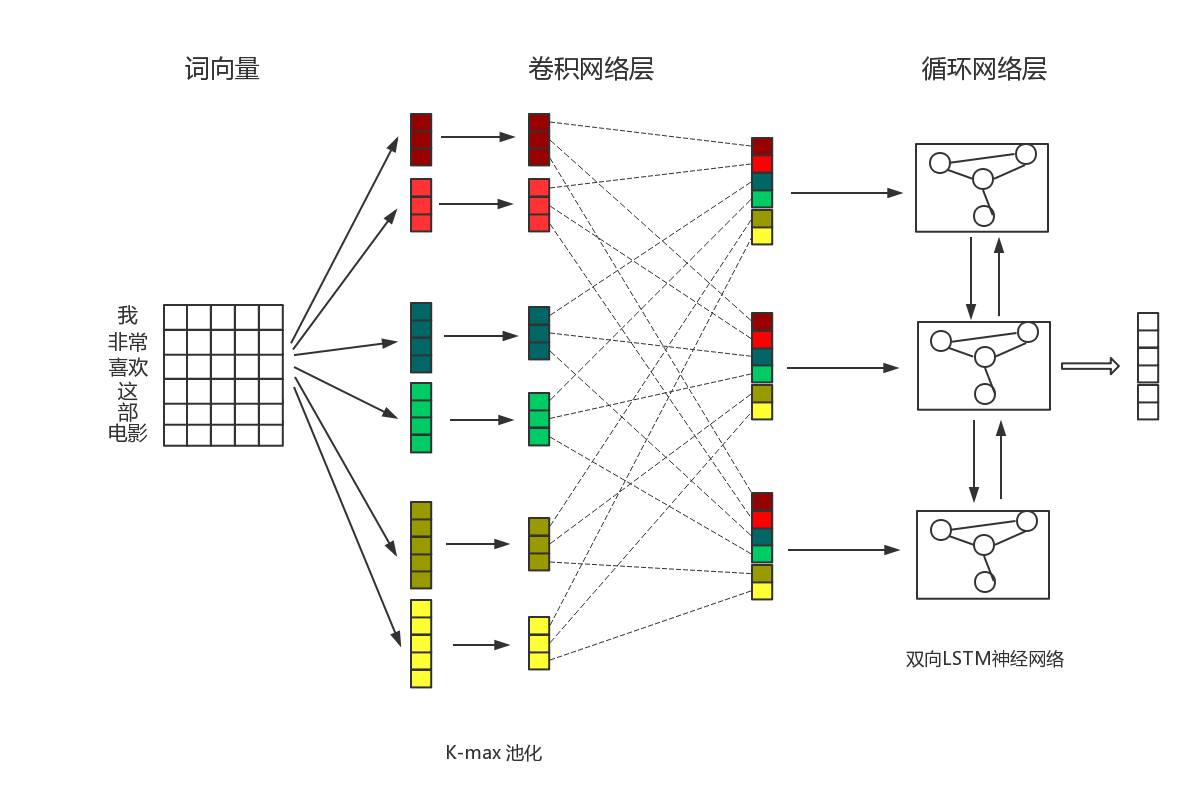
\includegraphics[scale=0.35]{picture/CLSTM.png}
    \caption{卷积循环神经网络结构图}
    \label{CLSTM}
\end{figure}
\subsection{卷积网络层}
卷积网络层的结构与普通卷积神经网络大致相同,分为卷积模块、池化模块与光栅模块。
为了适应本文研究的中文短文本数据,本文对每个模块的具体实现做出了一些调整,下面
对各个模块进行说明:

(1)卷积模块

基于文本数据的信息特征,卷积网络层的卷积模块使用窄卷积(Narrow Convolution)
作为卷积策略,避免宽卷积(Wide Convolution)的补零操作对提取文本特征造成影响。
由于短文本语料长度的特征,卷积核长度不宜过长,
本文中的卷积核设置为三种不同的长度,宽度为词向量的长度,
这样可以保证特征图能够覆盖尽可能多的文本特征。
每种卷积核生成128个,保障特征图的多样性。

(2)池化模块

由于短文本数据的长度以及卷积核的长度并不统一,卷积层产生的特征图的长度各有不同,
为了让接下来的循环网络层能够处理特征图,需要在池化模块对其进行处理,将长度统一。
本文使用k-max池化(k-max pooling)作为
池化算法,该算法是Kalchbrenner提出的动态k-max算法的前置算法\citing{kalchbrenner2014convolutional},
主要思想是对于一个给定的$k$值与特征序列$p$($p\in R^p,length(p)\geq k$),选择序列$p$中前$k$个最大值,
且保留原来序列的次序(即生成序列是原序列$p$的一个子序列)。通过k-max池化算法,卷积网络层不仅能够
接收变长的输入,同时生成的特征图也保留了相对的位置信息,提升了特征的质量。

(3)光栅模块

光栅模块主要用来整合生成的各个特征图,将其中相同位置的特征值进行合并,形成最终的特征向量,输入下面的循环网络层,
如网络结构图\ref{CLSTM}中的虚线所示。

\subsection{循环网络层}

循环神经网络依据时间对序列数据进行建模,上一个节点的数据不仅会进行输出,还会作为同一隐藏层下一个节点的输入,
隐藏层最后一个节点则能够接收到全部的文本特征数据。但是短文本分类任务需要更多的考虑文本上下文信息,单纯使用正向
循环神经网络,模型只能够依据上文信息进行分类,无法利用下文的信息,从而影响最终的分类效果。因此,本文使用
双向长短时记忆循环神经网络(Bi-directional Long Short-Term Memory,Bi-LSTM)作为循环网络层的实现,
将网络分为前向传递层与后向传递层,分别获取输入短文本的上文信息与下文信息,如图\ref{CLSTM}中的循环网络层所示。

Bi-LSTM网络的整体流程如图\ref{Bi-LSTM}所示,对于从上层网络传来的输入向量,网络首先将其转变为
正序序列及逆序序列两个向量,然后分别输入一个单向LSTM网络进行特征提取,得到正序特征向量与逆序特征向量,
之后将两个特征向量合并,形成最终的文本特征向量并输出到下一层网络。经过这样的处理,网络提取的特征向量既包含
上文信息又包含下文信息,能够给之后的分类网络提供更加丰富的语义信息,
一定程度上缓解了短文本数据语义信息不足的问题。
\begin{figure}[h]
    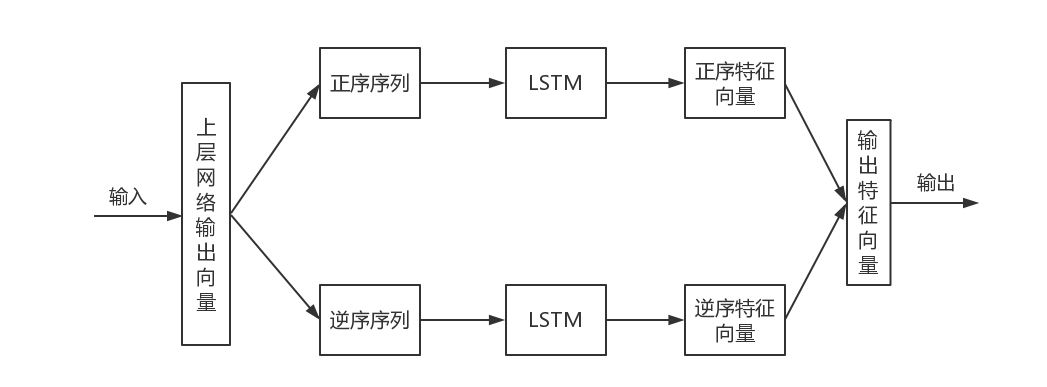
\includegraphics[scale=0.4]{picture/Bi-LSTM.png}
    \caption{Bi-LSTM网络流程图}
    \label{Bi-LSTM}
\end{figure}

\section{Attention-Based字词结合卷积循环中文短文本分类网络}
\subsection{Attention-Based卷积循环特征提取网络}
\label{ACLSTM_section}
根据Attention Model的思想,
本文改进了\ref{CLSTM_section}小节提出的卷积循环特征提取网络,
增加注意力权重,优化原始网络产生的特征向量。

Attention Model的核心在于注意力权重的获取,有多种实现方式,如Soft Attention、
Hard Attention等\citing{xu2015show}。为了减少模型的计算负担,
本文选择参数化的Soft Attention实现方式,该实现方式能够让整个Attention层直接嵌入
模型,使梯度可以经过Attention Mechanism模块,反向传播到其他地方,以此简化模型的训练过程。
总体计算流程如图\ref{Soft_Attention}所示,
首先把双层LSTM的输出$h$($h=\left \{ h_1,h_2,..,h_n\right\}$)
送入一个单层全连接神经网络,根据\ref{attention_eqn1}公式将其转换为中间向量$u$,
作为原始输出$h$的隐藏表示。
\begin{equation}
    u_i=\tanh\left ( W_wh_i+b_w \right )
    \label{attention_eqn1}
\end{equation}

然后通过softmax函数计算中间向量$u$与文本上下文向量$u_w$的相似度$\alpha$,如公式\ref{attention_eqn2}所示。
\begin{equation}
    \alpha_i=\frac{\exp\left ( u_{i}^{\top }u_w \right )}{\sum_n\exp\left ( u_{i}^{\top }u_w \right )}
    \label{attention_eqn2}
\end{equation}

其中$u_w$是记忆向量,可以视为筛选重要特征的高层抽象参数,代表着
整个语料库的上下文信息\citing{sukhbaatar2015end},在模型初始阶段随机初始化,
并在训练时同其他参数一起调整。计算结果$\alpha$则是标准化的注意力权重,用于下一步计算。

最后,把原始向量$h$和$\alpha$加权相加,就得到Attention优化后的特征向量$S$,如公式\ref{attention_eqn3}所示。
\begin{equation}
    S_i=\sum_n\alpha_ih_i
    \label{attention_eqn3}
\end{equation}
\begin{figure}[h]
    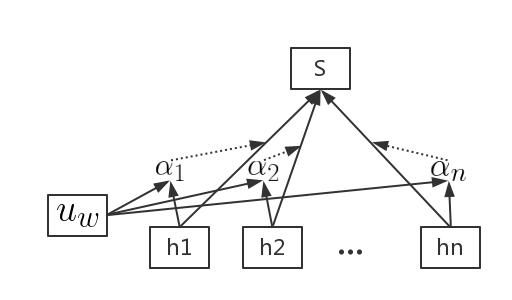
\includegraphics[scale=0.5]{picture/Attention.png}
    \caption{Soft Attention计算流程}
    \label{Soft_Attention}
\end{figure}

\subsection{双通道字词结合短文本分类模型}
在短文本分类任务中,词向量与字向量都能够作为文本的向量表示,但都有其固有的缺点:
词向量极度依赖分词结果,错误的分词会极大的影响词向量的性能;字向量虽然不存在分词的问题,但有些词语和
内部的汉字意思可能南辕北辙,如“东西”与其内部的汉字“东”和“西”,单纯从字向量很难推测出词的含义。
为了解决这个问题,本文设计了双通道字词结合短文本分类模型,同时接受短文本的词向量表示与字向量表示,
充分结合两者的特征信息,克服了常规分类模型的不足。

\begin{figure}[h]
    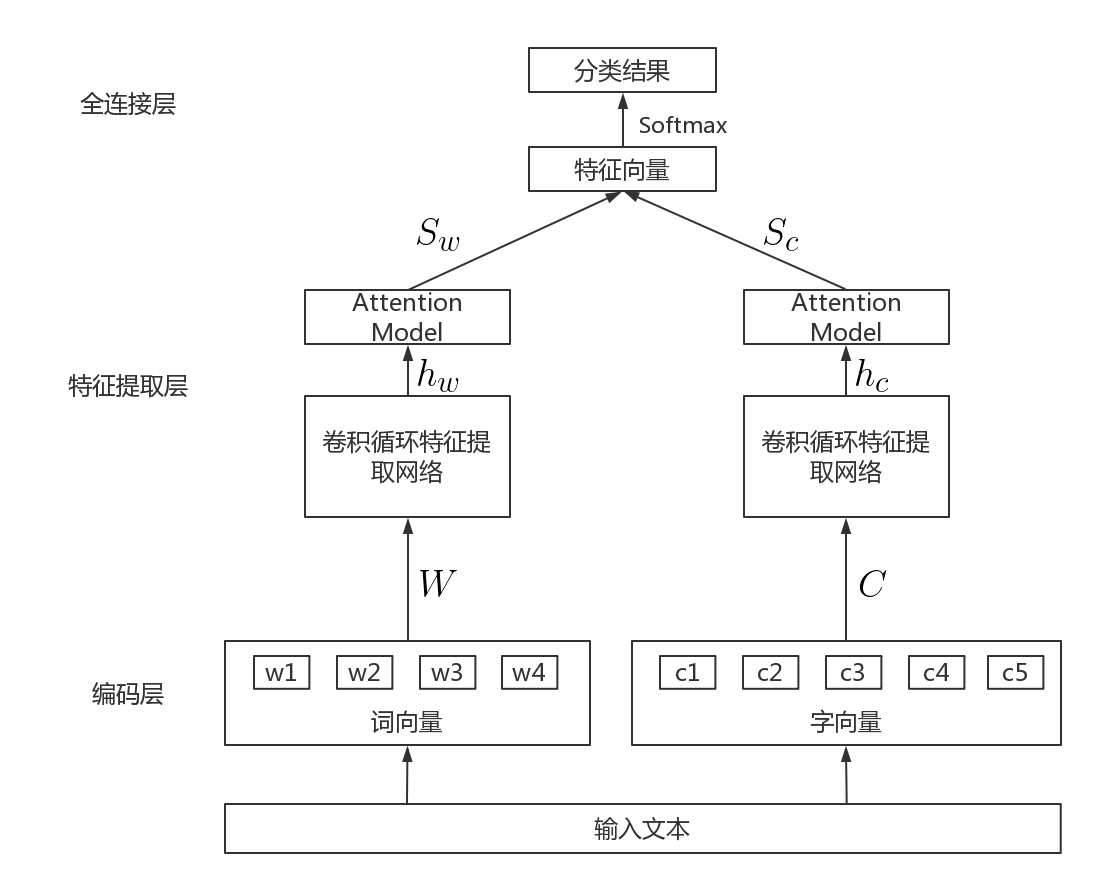
\includegraphics[scale=0.4]{picture/classifier.png}
    \caption{双通道字词结合短文本分类模型}
    \label{classifier}
\end{figure}

双通道字词结合短文本分类模型主要是构建一个包含两个平行的特征提取网络的分类模型,分别提取词向量特征与字向量特征,
总体结构如图\ref{classifier}所示。

模型总共分为三层:编码层、特征提取层与全连接层。编码层根据相应的词向量与字向量模型,将输入文本解析为词向量序列$W$
和字向量序列$C$。特征提取层分为两个平行的神经网络模块,由前文中的Attention-Based卷积循环特征提取网络组成,
分别提取词向量序列和字向量序列的文本特征,即向量$S_w$、$S_c$,然后根据公式\ref{classifier_eqn}将其合并,得到最终的文本特征向量$S$。
\begin{equation}
    S =\left [ S_w\bigoplus S_c \right ]
    \label{classifier_eqn}
\end{equation}

全连接层由线性转换层和Softmax层组成,其中线性转换层将特征向量$S$转换为一个维度与分类类别相当的实值向量,然后
Softmax层将这些实值映射为最终的条件概率,计算公式如\ref{softmax_eqn}所示。
\begin{equation}
    P=softmax\left ( W_sS+b_s \right )
    \label{softmax_eqn}
\end{equation}

本文使用公式\ref{cost_function}作为模型的损失函数,来最小化模型的分类误差。其中$N_t$表示训练语料库大小,
$N_c$表示类别数量,$P_{j}^{g}\left ( s_i \right )$表示当前文本的真实类别为$j$的概率,属于类别$j$则为1,否则为0。
%并且使用随机梯度下降算法(Stochastic Gradient Descent,SGD)作为训练的优化算法。
\begin{equation}
    Loss=-\sum_{i=1}^{N_t}\sum_{j=1}^{N_c}P_{j}^{g}\left ( s_i \right )\cdot\log\left ( P_j\left ( s_i \right ) \right )
    \label{cost_function}
\end{equation}
\section{实验设计和结果分析}
为了验证Attention-Based字词结合卷积循环中文短文本分类网络模型的可行性及有效性,本文
设计并实现了字向量/词向量两类总计8组对比实验模型,对新闻标题数据进行分类,并对结果进行分析。
\subsection{实验语料数据}
本实验所用的短文本数据由两部分组成,一部分来自“今日头条”网站,
另一部分为清华大学THUCTC新闻语料\citing{li2007scalable}。
语料库总计包含830396条新闻标题数据,共分为财经、科技、体育等12个类别(具体信息如表\ref{train_data_table}所示),
长度都在60字以内。
实验随机抽取80\%数据作为模型训练数据集,另外20\%则为验证集。
\begin{table}[h]
    \caption{实验语料库分类详情}
    \begin{tabular}{|c|c|c|c|}
        \hline
        类别 & 数量 & 类别 & 数量 \\
        \hline
        社会 & 57860 & 体育 & 134680 \\
        \hline
        时政 & 62658 & 股票 & 149853 \\
        \hline
        教育 & 41827 & 娱乐 & 92886 \\
        \hline
        财经 & 41085 & 家居 & 32188 \\
        \hline
        游戏 & 24313 & 房产 & 18440 \\
        \hline
        时尚 & 13150 & 科技 & 161456 \\
        \hline
    \end{tabular}
    \label{train_data_table}
    \end{table}

\subsection{实验环境及相关工具}
本实验模型采用机器学习库Tensorflow作为分类模型的实现工具。Tensorflow是
Google公司与2015年11月9日发布并宣布开源的机器学习框架,是现在最流行的深度学习项目之一。
Tensorflow支持Linux平台、Windows平台、Mac平台等多种主流平台,提供了非常丰富的
深度学习相关API,包括基本的向量矩阵计算、各种优化算法、
各种卷积神经网络和循环神经网络基本单元的实现、
以及可视化的辅助工具等等。
Tensorflow将所有用户输入的计算结构都视为数据流图(data flow graphs),图中的
节点(nodes)表示数学操作,连接节点的线表示在节点间相互输送数据的多维数据数组,
即张量(tensor)。
Tensorflow可以适应任何硬件环境,无论台式机、服务器、手机移动设备都可以
直接运行计算代码,并且拥有自动求微分功能,在模型训练时自动计算相关的微分导数,极大的简化了
深度学习代码的开发。

本实验使用英伟达GeForce显卡作为模型训练的辅助工具。
通过英伟达推出的CUDA技术(Compute Unified Device Architecture,统一计算架构),
使用GeForce显卡能够在在GPUs(GPGPU)上使用图形APIs进行传统通用计算,从而加速模型训练。

本实验具体的实验环境如表\ref{train_env_table}所示:
\begin{table}[h]
    \caption{实验环境具体配置}
    \begin{tabular}{|c|c|}
        \hline
        操作系统 & Ubuntu 16.04 \\
        \hline
        开发语言 & Python 3.6 \\
        \hline
        开发平台 & Google Tensorflow深度学习框架 \\
        \hline
        CPU & Intel I5 \\
        \hline
        内存 & 8G \\
        \hline
        硬盘 & 1T \\
        \hline
        显卡 & NVIDIA GeForce 1080 \\
        \hline
    \end{tabular}
    \label{train_env_table}
\end{table}
\subsection{分类模型评价方法}
\label{test_fun}
分类模型的有效性有多种评价方法,如准确率(Precision)、
召回率(Recall)和F1-Measure。对于分类模型的分类结果,总体可以分为4中情况,如表\ref{classification_demo_table}所示。
\begin{table}[h]
    \caption{分类结果示例表}
    \begin{tabular}{|c|c|c|}
        \hline
        & 实际属于该类 & 实际不属于该类 \\
        \hline
        被分到该类 & TP & FP \\
        \hline
        未被分到该类 & FN & TN \\
        \hline
    \end{tabular}
    \label{classification_demo_table}
\end{table}
其中TP表示实际属于该类且被模型分到该类的样例数。FP表示实际不属于该类,但被
模型分到该类的样例数。FN表示实际属于该类,但未被分到该类的样例数。TN表示实际不属于该类,
且未被分到该类的样例数。

根据表\ref{classification_demo_table},准确率计算公式可写为式\ref{accuracy}。
\begin{equation}
    Accuracy=\frac{TP+TN}{TP+FP}
    \label{accuracy}
\end{equation}
召回率可定义为式\ref{recall}。
\begin{equation}
    Recall=\frac{TP+TN}{TP+FN}
    \label{recall}
\end{equation}
准确率反映了模型分类结果的正确率,召回率反映了模型找到正确类别的能力,两者都可以
体现分类模型有效性,但很多时候会相互矛盾。为了正确评价本实验中实现的所有模型,本文使用
这两个的加权调和平均值作为评价标准,即F1-Measure,计算公式如\ref{f1-measure}所示。
\begin{equation}
    F1-Measure=\frac{2\times Precision \times Recall}{Precision+Recall}
    \label{f1-measure}
\end{equation}
\subsection{对比实验设计}
为了验证本文设计的模型对于短文本分类的效果,本实验设计了4组对比实验,每组又词向量分类模型与
字向量分类模型两种,总计8个对比实验:

(1)传统LSTM模型

模型结构与实现方式由文献\cite{zhou2016compositional}提供,
词向量版本使用Ansj中文分词开源库以及word2vec工具将训练语料映射为200维的词向量文本数据,
字向量版本使用word2vec工具将训练语料映射为200维的字向量文本数据。隐藏层的节点个数设置为200。
模型训练的学习率(learn rate)取0.001,优化算法使用随机梯度下降算法(Stochastic Gradient Descent,SGD)。
分类器使用多类分类的逻辑回归分类器,使用LSTM模型隐藏层最后一个节点的输出值作为分类特征向量。训练循环次数为50,
批尺寸(batch size)为200。

(2)传统CNN模型

模型结构与实现方式同样由文献\cite{zhou2016compositional}提供,
词向量版本使用Ansj中文分词开源库以及word2vec工具将训练语料映射为200维的词向量文本数据,
字向量版本使用word2vec工具将训练语料映射为200维的字向量文本数据。卷积层使用大小为3、4、5的三类卷积核,每类卷积核的个数为128。
池化层使用最大池化算法。
模型训练的学习率取0.001,优化算法使用随机梯度下降算法。
分类器使用多类分类的逻辑回归分类器。训练循环次数为50,
批尺寸为200。

(3)传统卷积循环网络模型(CLSTM)

模型依据文献\cite{Zhou2015A}实现,
词向量版本使用Ansj中文分词开源库以及word2vec工具将训练语料映射为200维的词向量文本数据,
字向量版本使用word2vec工具将训练语料映射为200维的字向量文本数据。
卷积层使用大小为3、4、5的三类卷积核,每类卷积核的个数为128。
池化层使用最大池化算法。
LSTM层的隐藏节点个数设置为200。
模型训练的学习率取0.001,优化算法使用随机梯度下降算法。
分类器使用多类分类的逻辑回归分类器。训练循环次数为50,
批尺寸为200。

(4)Attention-Based卷积循环网络模型(Attention-CLSTM)

模型依据\ref{ACLSTM_section}小节的设计实现,
词向量版本使用Ansj中文分词开源库以及word2vec工具将训练语料映射为200维的词向量文本数据,
字向量版本使用word2vec工具将训练语料映射为200维的字向量文本数据。
卷积层使用大小为3、4、5的三类卷积核,每类卷积核的个数为128。
池化层使用k-max池化算法。
LSTM层的隐藏节点个数设置为200。
Attention层隐藏参数向量长度为200。
模型训练的学习率取0.001,优化算法使用随机梯度下降算法。
分类器使用多类分类的逻辑回归分类器。训练循环次数为50,
批尺寸为200。

本文设计的分类模型同时使用词向量文本数据与字向量文本数据,都为200维。两个通道的
卷积层都使用大小为3、4、5的三类卷积核,每类卷积核的个数为128,池化层都使用k-max池化算法,
LSTM层的隐藏节点数目与Attention层的隐藏参数向量长度也都为200。
模型训练的学习率取0.0001,优化算法使用随机梯度下降算法。
分类器使用多类分类的逻辑回归分类器。训练循环次数为50,
批尺寸为200。
\subsection{实验结果和分析}
本文对上一个小节设计的实验模型在新闻标题语料库上进行实验,
每个模型都训练5次并选取平均结果。
实验对比结果如表\ref{classification_result_table}所示。
\begin{table}[h]
    \caption{实验对比结果}
    \begin{tabular}{|c|c|c|}
        \hline
        模型 & 词向量 & 字向量 \\
        \hline
        传统CNN & 0.855679 & 0.835943 \\
        \hline
        传统LSTM & 0.869336 & 0.849313 \\
        \hline
        CLSTM & 0.894824 & 0.872391 \\
        \hline
        Attention-Based CLSTM & 0.89947 & 0.87346 \\
        \hline
        双通道Attention-Based CLSTM(本文设计) & \multicolumn{2}{|c|}{0.913441} \\
        \hline
    \end{tabular}
    \label{classification_result_table}
\end{table}

从实验结果中可以看出,虽然传统CNN能够动态获取文本的本地特征,
但由于忽略了特征的位置信息,因此分类效果不如其他模型。
传统LSTM模型因为其结构的特点,对文本数据建模更有成效,随意相比传统CNN模型效果
有所提升。CLSTM模型则将上述两个模型进行了融合,两种结构起到了互补的作用,
因此分类效果有了较大提升,达到了0.894824与0.872391。
Attention-Based CLSTM模型同样融合了CNN与LSTM网络,但与CLSTM模型不同的是,
模型中添加的Attention Model在分类器之前对文本特征向量做了一次筛选,
所以分类效果有了一定提升。并且,对比表格中的词向量结果与字向量结果,可以发现
使用词向量的分类模型全部优于使用字向量的分类模型,这说明对于中文文本,词向量
仍然是文本信息的主要来源,字向量虽然也能达到还算满意的分类效果,但在文本的表现力
上还是不如词向量优秀。本文设计的双通道Attention-Based CLSTM分类模型
在Attention-Based CLSTM模型的基础上增加了字向量数据通道,通过
综合词向量与字向量文本特征的方式,得到了比单独使用语义更加丰富的特征向量,
在实验中取得了最好的结果。
\section{本章小结}
本章主要提出了Attention-Based字词结合卷积循环中文短文本分类模型。
首先介绍了用于提取文本特征的卷积循环神经网络,然后再结合Attention Model的相关
概念提出了Attention-Based卷积循环神经网络。之后加入字向量数据,设计了一个双通道的短文本分类模型,
弥补了使用单一词向量/字向量的不足。
最后通过对比实验,验证了模型的可行性及有效性。
    \chapter{短文本分类系统设计和实现}
本章主要阐述短文本分类系统的功能设计与代码实现,并详细介绍系统包含的各个功能模块。
整个系统可以分为离线网络训练与在线短文本分类两大部分,离线网络训练用于语料库更新以及
分类模型学习与参数调优,在线短文本分类则是系统实际提供的功能,用于给外部系统调用。
这两部分相互依赖,只有通过离线网络训练不断更新分类模型数据,
在网络训练时将模型参数调整到最优,才能让在线分类系统获得最好的效果。
\section{系统总体概述}
该短文本分类系统设计的主要目的是给其他用户提供一个持续可靠的短文本分类服务,主要思想是依据使用领域不断通过网络爬虫
搜集标注好的训练语料,训练出相应的词向量与字向量。然后系统使用这些文本表示信息训练分类
网络,并根据在验证集上的表现动态调节相关参数让模型效果达到最优。最后使用训练得到的网络参数
给前台用户提供短文本分类服务。系统的总体架构逻辑上大致可以分为三个子系统:
训练语料更新子系统、分类模型训练子系统和短文本分类子系统,整个流程如图\ref{system_architecture}所示。
\begin{figure}[h]
    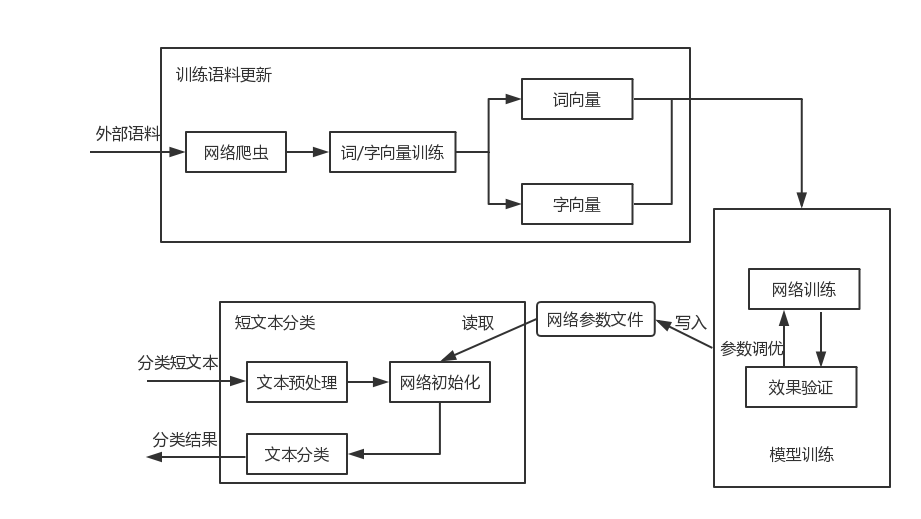
\includegraphics[scale=0.45]{picture/system_architecture.png}
    \caption{短文本分类系统流程}
    \label{system_architecture}
\end{figure}

为了保证系统的运算速度以及服务的稳定性,后台的语料更新子系统和短文本分类子系统都由包含多台
计算机的集群提供服务,分类模型训练子系统则为高性能运算服务器,配备有能够加速矩阵、向量计算
的NVIDIA Geforce显卡。系统的整体物理部署如图\ref{system_deployment}所示。
\begin{figure}[h]
    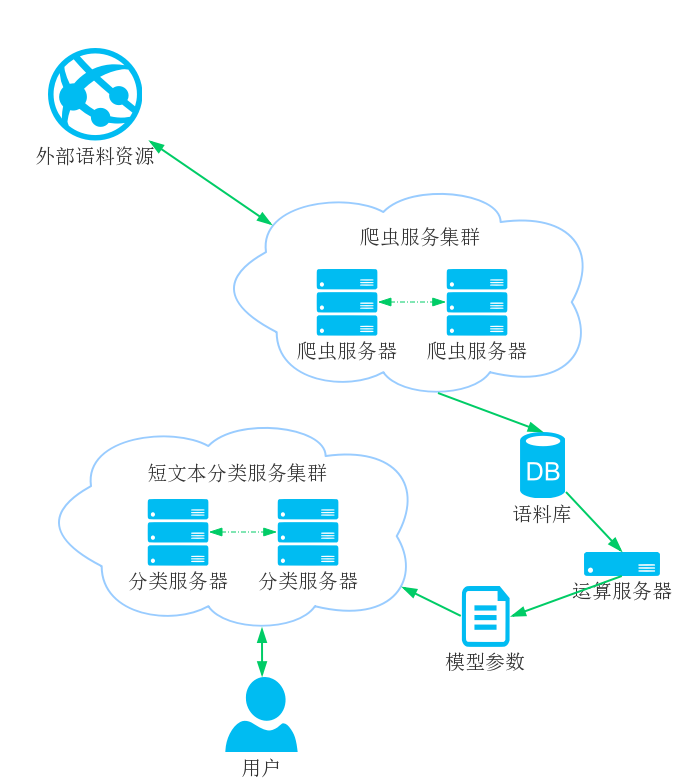
\includegraphics[scale=0.45]{picture/system_deployment.png}
    \caption{分类系统物理部署}
    \label{system_deployment}
\end{figure}
\section{系统各模块的设计和实现}
系统各个子系统的功能模块如图\ref{system_module}所示,训练语料更新子系统分为
网络爬虫、队列管理、语料数据存储、词/字向量训练四个模块,模型训练子系统分为
分类网络训练、参数调优两个模块,短文本分类子系统分为分类服务、日志记录两个模块。
其中训练语料更新子系统和模型训练子系统为后台模块,由系统定时启动,用于实时更新系统的
模型参数,短文本分类子系统为前台模块,用于与用户交互,给外部用户提供短文本分类服务。
下面对每一个功能模块进行详细阐述。
\begin{figure}[h]
    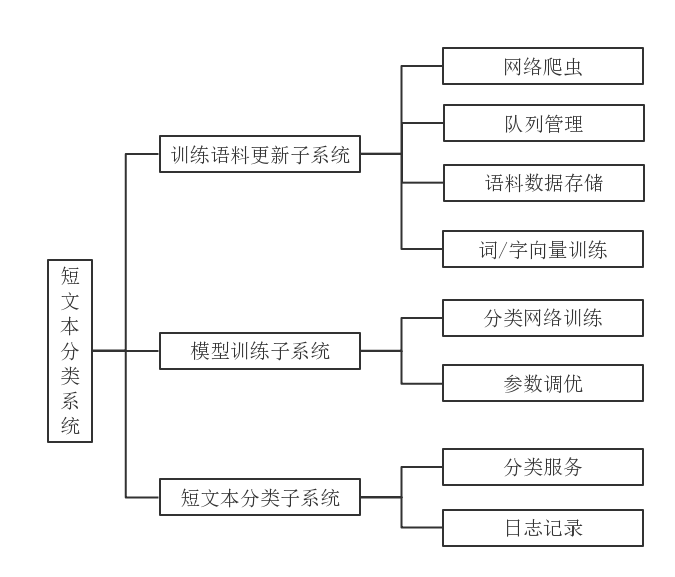
\includegraphics[scale=0.45]{picture/system_module.png}
    \caption{系统功能模块图}
    \label{system_module}
\end{figure}
\subsection{网络爬虫}
网络爬虫模块采用分布式爬虫架构,由多个网络节点中的爬虫程序共同完成数据抓取任务。
爬虫程序基于Python的Scrapy框架开发,
该框架是一个快速、
高层次的屏幕抓取和web抓取框架,用于抓取web站点并从页面中提取结构化的数据,
并且轻量灵活,能够快速的二次开发,适应不同爬虫需求。
\begin{figure}[h]
    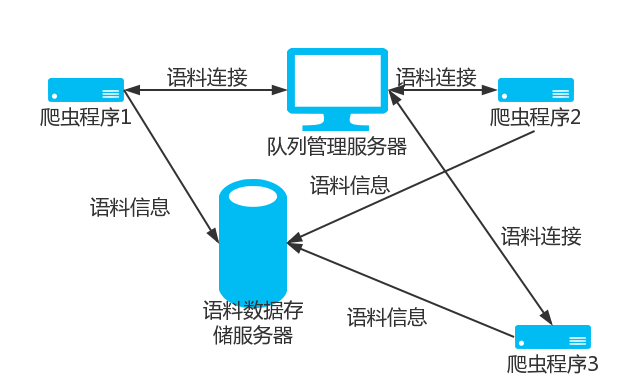
\includegraphics[scale=0.5]{picture/spider.png}
    \caption{网络爬虫模块结构图}
    \label{spider}
\end{figure}

爬虫模块的整体结构如图\ref{spider}所示,爬虫任务由队列管理模块分发,爬虫程序
负责数据的获取,然后将获取的数据写入语料数据存储模块。
每个爬虫程序包含4个组件:
\begin{itemize}
    \item[-] 下载器:负责通过http/https协议从外部WEB服务器下载WEB页面,以便后续的处理。
    \item[-] 页面解析器:负责解析下载的WEB页面,抽取所需的信息,以及发现新的语料链接并发送到队列管理模块。
    \item[-] 存储器:负责将获取的有用信息存储到语料数据存储模块。
    \item[-] IP池:负责给下载器提供代理IP,防止外部WEB服务器感知并禁止爬虫模块的请求。
\end{itemize}
\begin{figure}[!hbp]
    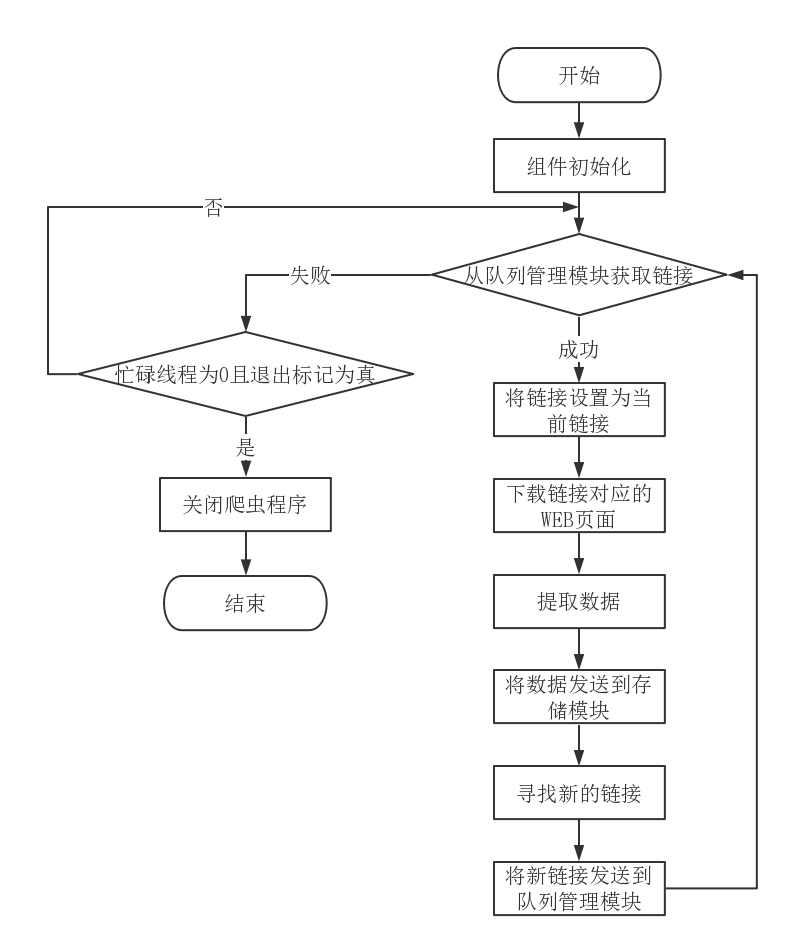
\includegraphics[scale=0.4]{picture/spider_flowchart.png}
    \caption{爬虫程序运行流程}
    \label{spider_flowchart}
\end{figure}

爬虫程序运行流程如图\ref{spider_flowchart}所示,首先,程序对各个组件进行初始化工作,
如生成下载器、设置线程池线程数量等。初始化结束之后,程序的主线程开始尝试从队列管理模块获取
下载链接,如果获取成功,则生成一个Task任务块并将其设置为当前任务,然后从线程池中取出一个线程进行下一步的处理,
如果获取失败,则认为当前任务可能已经结束,并检测退出标志是否为真以及是否还有工作中的线程,
两者都为真时表示系统已经确定退出,程序会立即关闭线程池,结束工作。
子线程接收到Task任务块会立刻运行下载器下载对应的WEB页面,下载完成后则通过页面解析器进行解析,然后
将解析得到的所需数据以及新的连接分别发送到语料信息存储模块和队列管理模块。
爬虫程序的核心页面处理代码如下所示:
\begin{lstlisting}[language={Python},frame=shadowbox,rulesepcolor=\color{red!0!green!0!blue!0}] 
    def parse(self, response):
    news = json.loads(response.body.decode('utf-8'))
    if news["message"] == "error":
        # 服务器返回错误数据,当前IP地址可能被禁止
        if "proxy" in response.meta:
            self.ban_ip[response.meta["proxy"]] = 1
        else:
            self.ban_ip[""] = 1
        print("ban ip: " + str(len(self.ban_ip)) + "/" + str(len(IP_POOL)))
        if len(self.ban_ip) >= len(IP_POOL):
            raise CloseSpider("ban")
        yield Request(response.url, dont_filter=True)
    else:
        # 获取新闻语料
        news_list = news["data"]
        for news_item in news_list:
            item = NewsSpiderItem()
            if "chinese_tag" not in news_item or news_item["chinese_tag"] == "其他" or \
               news_item["chinese_tag"] == "视频":
                continue
            item["tag"] = news_item["chinese_tag"]
            item["title"] = news_item["title"]
            item["hash"] = self.__get_md5(news_item["title"].encode("utf-8"))
            # 返回获取的数据
            yield item
        next_time = news["next"]["max_behot_time"]
        sign = lib.get_sign(next_time)
        ascp_dict = lib.get_as_cp()
\end{lstlisting}
\begin{lstlisting}[language={Python},frame=shadowbox,rulesepcolor=\color{red!0!green!0!blue!0}] 
        # 返回新发现的链接
        yield Request(self.api_format % (self.__get_url_tag(response.url), next_time, next_time,
                                         ascp_dict["as"], ascp_dict['cp'], sign))
\end{lstlisting}
\subsection{队列管理}
队列管理模块主要用来给整个爬虫网络提供一个可靠的任务管理服务,统一分发数据爬取任务,
平衡各节点的工作负担,负载均衡,防止忙碌节点的出现。模块以稳定性、实时性较好的
Redis(REmote DIctionary Server)分布式数据库为基础实现,通过将爬虫程序
上传的新链接重新分配给网络中的其他节点,不断推进整体的数据爬取进度,工作示意图大致
如图\ref{redis}所示。
\begin{figure}[h]
    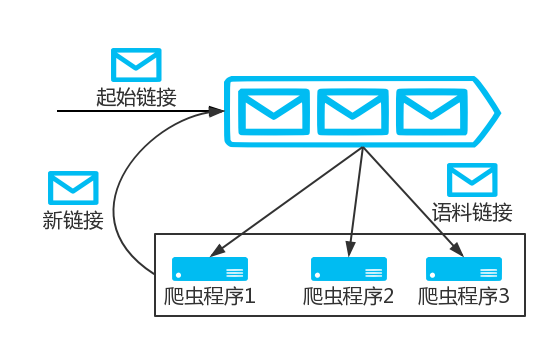
\includegraphics[scale=0.5]{picture/redis.png}
    \caption{队列管理模块工作示意图}
    \label{redis}
\end{figure}
\subsection{语料数据存储}
语料数据存储模块用于持久化保存爬虫程序提取的语料信息,使用Mysql数据库实现。
为了获取语料的全面信息,语料数据存储模块除了存储语料文本,还存储了来源、URL链接、
发布时间、爬取时间、文本MD5等重要信息,以新闻标题语料为例,相关数据格式如表\ref{news_struct_table}所示,
爬取的相应数据见表\ref{news_data_table}所示。

\begin{table}[h]
    \caption{新闻标题语料数据格式}
    \begin{tabular}{|c|c|c|c|}
        \hline
        title & 新闻的标题 & url & 新闻的url地址 \\
        \hline
        time & 新闻的发布时间 & get\_time & 新闻的爬取时间 \\
        \hline
        resource & 新闻的来源 & news\_id & 新闻的id \\
        \hline
        news\_md5 & 新闻标题文本的md5值 & category & 新闻所属的类别  \\
        \hline
    \end{tabular}
    \label{news_struct_table}
    \end{table}

\begin{table}[h]
    \caption{爬取的新闻标题数据}
    \begin{tabular}{|c|c|}
        \hline
        title & 男子出狱创业招500名犯人,为帮员工戒毒半年吃素 \\
        \hline
        url & http://toutiao.com/group/6504029172468285966/ \\
        \hline
        time & 1511756299 \\
        \hline
        get\_time & 1511759149 \\
        \hline
         category & 社会 \\
        \hline
        resource & 人民网 \\
        \hline
        news\_id & 6504029172468285966 \\
        \hline
        news\_md5 &  1ce5761e192c42e76e4bb45ac22be5ed \\
        \hline
    \end{tabular}
    \label{news_data_table}
    \end{table}

同时,为了后续模块能够方便的处理爬取的语料数据,存储模块还需要对这些数据进行预处理工作,
包括标点符号剔除、分词处理、繁简转换、分词筛选、去除停用词、汉字统计。
其中标点符号剔除、分词处理、繁简转换和之前小节介绍的一样,这里不再赘述,分词筛选是用于统计
语料中发现的新词,汉字统计则是统计新汉字,这两者是判断是否需要更新词向量/字向量的重要指标。去除停用词使用的是
哈工大、百度、川大的停用词列表,能够有效去除语料中对语义特征没有帮助的词。同样以新闻标题数据为例,
预处理之后的数据如表\ref{pretreatment_data_table}所示。
\begin{table}[h]
    \caption{预处理过后的新闻数据}
    \begin{tabular}{|c|c|}
        \hline
        id & 1303086993 \\
        \hline
        news\_id & 6504029172468285966 \\
        \hline
        words & 男子,出獄,創業,招,犯人,幫,員工,戒毒,半,年,吃,素 \\
        \hline
        char & 男,子,出,獄,創,業,招,犯,人,幫,員,工,戒,毒,半,年,吃,素 \\
        \hline
    \end{tabular}
    \label{pretreatment_data_table}
    \end{table}
\subsection{字/词向量训练}
字/词向量训练模块主要用来获取分类模型使用的词向量与字向量,采用增量训练的方式,
只有在语料数据或新词/新字数量超过一定阈值的时候,才开始训练,更新当前使用的词/字向量。

由\ref{recwe_section}节的目标公式以及负采样算法可以继续推导得式\ref{neg_eqn}:
\begin{equation}
    \begin{aligned}
        L &= \sum_{w\in l}\sum_{u\in \left \{ w \right \}\cup NEG\left ( w \right )}\left \{ L^w\left ( u \right ) \cdot \log \left [ \sigma \left ( X_w^{\top }\theta^u  \right ) \right ]+\left [ 1-  L^w\left ( u \right )\right ]\cdot \log \left [1- \sigma \left ( X_w^{\top }\theta^u  \right ) \right ]\right \} \\
        &+ \sum_{c\in l}\sum_{u\in \left \{ c \right \}\cup NEG\left ( c \right )}\left \{ L^c\left ( u \right ) \cdot \log \left [ \sigma \left ( X_c^{\top }\theta^u  \right ) \right ]+\left [ 1-  L^c\left ( u \right )\right ]\cdot \log \left [1- \sigma \left ( X_c^{\top }\theta^u  \right ) \right ]\right \}
    \end{aligned}
    \label{neg_eqn}
\end{equation}

再根据式\ref{neg_eqn}分别对各个参数求导,即可得到词向量/字向量的梯度更新方法,如公式所示\ref{neg_update_eqn}。
\begin{equation}
    \begin{aligned}
        q&=\sigma \left ( X_w^\top \theta^u \right )\\
        g&=\eta \left ( L^w\left ( u \right )-q \right )\\
        e &:=e+g\theta^u\\
        \theta^u &:=\theta^u+gX_w\\
        v_u &:=v_u+e
    \end{aligned}
    \label{neg_update_eqn}
\end{equation}

词/向量训练代码由C语言实现,核心部分分为正向推导、梯度计算、反向更新三个部分。
正向推导主要是从模型底部统计所有输入向量,得到当前预测的隐藏层向量,对应的代码如下所示:
\begin{lstlisting}[language={[ANSI]C},frame=shadowbox,rulesepcolor=\color{red!0!green!0!blue!0}] 
    //叠加窗口内的词向量
    for(c = 0; c < layer1_size; c++) 
        neu1[c] += syn0[c + last_word * layer1_size];
    //叠加字向量
    for(c = 0; c < vocab[last_word].character_size; c++)
    {
        char_id = vocab[last_word].character[c];
        char_id_list[char_list_cnt++] = char_id;
        for(d = 0; d < layer1_size; d++) neucomp[d] += synchar[d + char_id * layer1_size];
        for(d = 0; d < char2comp[char_id].comp_size; d++)
        {
            comp_id = char2comp[char_id].comp[d];
            if(comp_id != char_id)
            {
                comp_id_list[comp_list_cnt++] = comp_id;
                //叠加部首向量
                for(e = 0; e < layer1_size; e++) neucomp[e] += synchar[e + comp_id * layer1_size];
            }
        }
    }
\end{lstlisting}

梯度计算部分是根据公式\label{neg_update_eqn}计算当前输入对应的梯度,代码如下所示。
\begin{lstlisting}[language={[ANSI]C},frame=shadowbox,rulesepcolor=\color{red!0!green!0!blue!0}] 
    
for(d = 0; d < negative + 1; d++)
{
    //一些初始化操作
    ...
    // 开始计算梯度
    l2 = target * layer1_size;
    real f1 = 0, f3 = 0, g1 = 0, g3 = 0;
    for(c = 0; c < layer1_size; c++)
    {
        f1 += neu1[c] * syn1neg[c + l2];
        f3 += neucomp[c] * syn1neg[c + l2];
    }
    //f1
    if(f1 > MAX_EXP)
        g1 = (label - 1) * alpha;
    else if(f1 < -MAX_EXP)
        g1 = (label - 0) * alpha;
    else
        g1 = (label - expTable[(int) ((f1 + MAX_EXP) * (EXP_TABLE_SIZE / MAX_EXP / 2))]) * alpha;

    //f3
    if(f3 > MAX_EXP)
        g3 = (label - 1) * alpha;
    else if(f3 < -MAX_EXP)
        g3 = (label - 0) * alpha;
    else
        g3 = (label - expTable[(int) ((f3 + MAX_EXP) * (EXP_TABLE_SIZE / MAX_EXP / 2))]) * alpha;
    // 统计梯度
    for(c = 0; c < layer1_size; c++)
    {
        neu1_grad[c] += g1 * syn1neg[c + l2];
        neucomp_grad[c] += g3 * syn1neg[c + l2];
    }
    //更新 syn1neg
    for(c = 0; c < layer1_size; c++)
        syn1neg[c + l2] += g1 * neu1[c] + g3 * neucomp[c];
    
}
\end{lstlisting}

反向更新部分则是用上个部分得到的梯度更新输入的词向量与字向量及部首向量,完成一次训练,相关代码如下所示:
\begin{lstlisting}[language={[ANSI]C},frame=shadowbox,rulesepcolor=\color{red!0!green!0!blue!0}] 
for(a = b; a < window * 2 + 1 - b; a++)
    if(a != window)
    {
        c = sentence_position - window + a;
        if(c < 0) continue;
        if(c >= sentence_length) continue;
        last_word = sen[c];
        if(last_word == -1) continue;
        for(c = 0; c < layer1_size; c++)
        {
            //更新词向量
            syn0[c + last_word * layer1_size] += neu1_grad[c] / cw;
        }
    }
    for(a = 0; a < char_list_cnt; a++)
    {
        char_id = char_id_list[a];
        for(c = 0; c < layer1_size; c++)
        {
            //更新字向量
            synchar[c + char_id * layer1_size] += neucomp_grad[c] / (char_list_cnt + comp_list_cnt);
        }
    }
    for(a = 0; a < comp_list_cnt; a++)
    {
        comp_id = comp_id_list[a];
        for(c = 0; c < layer1_size; c++)
        {
            //更新部首向量
            synchar[c + comp_id * layer1_size] += neucomp_grad[c] / (char_list_cnt + comp_list_cnt);
        }
    }
\end{lstlisting}
\subsection{模型训练}
模型训练子系统包含分类网络训练与参数调优两个模块,是整个系统的核心部分,用于训练并获取
分类性能最优的网络模型参数。详细过程设计如图\ref{train}所示。
\begin{figure}[!hbp]
    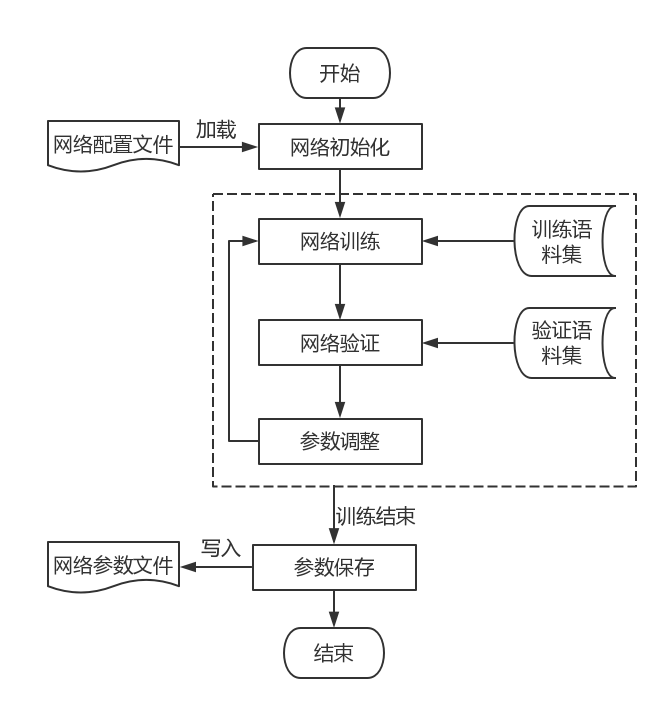
\includegraphics[scale=0.6]{picture/train.png}
    \caption{模型训练子系统过程示意图}
    \label{train}
\end{figure}

模型训练子系统的详细流程如下:
\begin{enumerate}
    \item 根据配置文件中的相关配置信息使用Google Tensorflow深度学习框架构建
    \ref{4_section}中提出的短文本分类网络结构。
    \item 使用误差反向传播算法(Error Back Propagation,BP)不断进行前向计算与后向
    传导,更新网络参数。
    \item 使用验证语料集对训练好的网络进行测试,确定网络的性能以及判断网络是否正确
    收敛。验证语料集不参与网络训练,仅仅在其上进行BP算法的前向过程。
    \item 根据相关配置文件,在一定范围内微调网络的参数并使用新参数重新训练玩了个,
    尝试优化网络。在调整一定次数之后,取性能最好的网络参数作为最后的有效参数。
    \item 保存完成调优之后的网络参数,以便后续阶段使用。
\end{enumerate}

表\ref{net_data_alert_table}展示了需要调节的网络参数及其调节范围,参数微调时会在范围内对相关参数重新取值。
图\ref{train_tmp_data}展示了系统保存的网络参数,训练过程中产生所有模型参数都会被保存并统一编号,方便日后管理
人员分析。
\begin{table}[h]
    \caption{微调参数列表}
    \begin{tabular}{|c|c|}
        \hline
        参数名称 & 调节范围 \\
        \hline
         LSTM隐藏层大小 & 64-256 \\
        \hline
        CNN卷积核数量 & 64-256 \\
        \hline
        CNN卷积核高度 & 2-10 \\
        \hline
        Dropout层丢弃率 & 0.2-0.6 \\
        \hline
        学习率 & 0.001-0.0001 \\
        \hline
        Attention层大小 & 65-256 \\
        \hline
    \end{tabular}
    \label{net_data_alert_table}
    \end{table}

\begin{figure}[!hbp]
    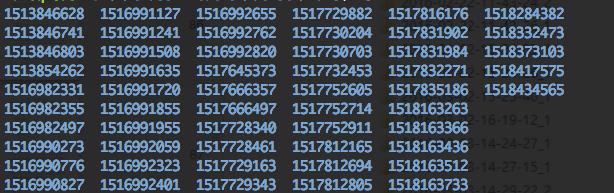
\includegraphics[scale=0.6]{picture/train_tmp_data.png}
    \caption{模型保存的网络参数文件}
    \label{train_tmp_data}
\end{figure}
\subsection{分类服务}
分类服务模块主要是给外部用户提供一个持续有效的即时短文本分类服务,
整个服务依托于HTTP协议,通过传递Json进行数据交换,外部用户只要按照格式要求
给系统发送JSON数据,系统即会返回分类结果。服务网络由多台服务节点组成,并使用
Nginx反向代理服务器提供链接分发服务,保证系统的稳定性以及可拓展性,具体框架如图\ref{server_chart}所示。
\begin{figure}[!hbp]
    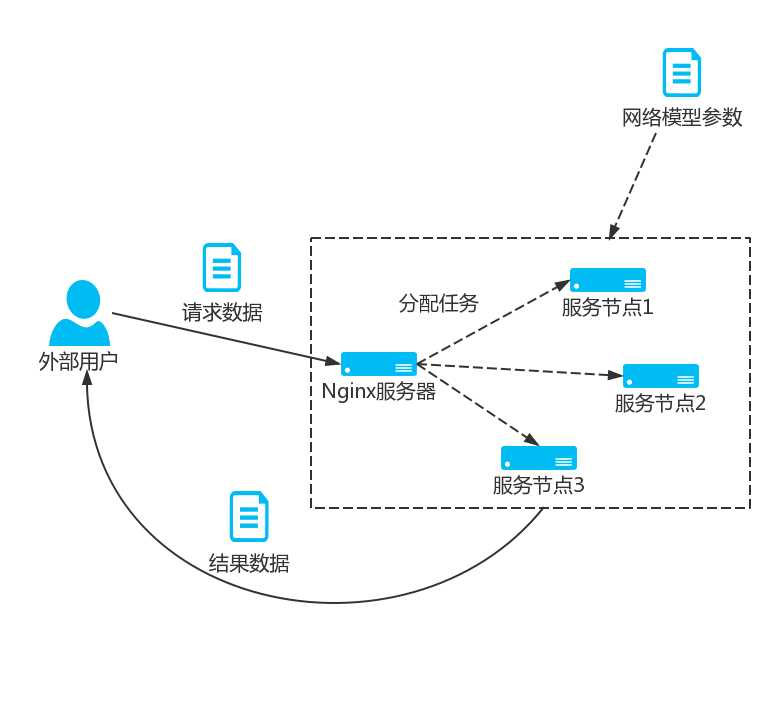
\includegraphics[scale=0.6]{picture/server_chart.png}
    \caption{分类服务模块基本框架示意图}
    \label{server_chart}
\end{figure}

用户的分类请求首先发往Nginx代理服务器,由代理服务器统一分配服务节点。服务节点接收到分类文本之后,
需要对其分词、去除标点与停用词,然后按照词/字向量表转换为对应的词向量/字向量数据,同时忽略词表/字表中没有词或字。
最后将数据送入分类网络,并将分类结果返回给用户。
\subsection{日志记录}
日志记录模块用于记录外部用户的相关信息,记录内容包括用户编号、用户IP、分类文本等,
同时系统的分类结果也会被保存,方便以后的查阅以及错误排查。日志存储模块使用Mongodb
作为存储数据库。Mongodb与常见的Mysql数据库等关系数据库不同,采用非关系结构存储数据,
同时侧重大量数据写入性能,非常适合日志信息存储。用户日志的具体信息如表\ref{log_table}所示。
\begin{table}[h]
    \caption{用户日志字段}
    \begin{tabular}{|c|c|}
        \hline
        字段名称 & 字段值 \\
        \hline
        \_id & ObjectId("41d2c2913761a2258c7c4e79") \\
        \hline
        user\_id & dca8815bef5e1150 \\
        \hline
        time & 2016-01-27 05:55 \\
        \hline
        model\_arg & 1517812805 \\
        \hline
        content & 如果一个人临去世之前把信用卡全部套现,银行会怎么办? \\
        \hline
        classification\_result & 财经 \\
        \hline
    \end{tabular}
    \label{log_table}
    \end{table}

\section{系统测试与分析}
为了验证系统的有效性以及在最新短文本语料数据上的分类效果,
需要在实际网络环境中进行系统测试,并对系统的测试结果进行统计、分析。
本文将在今日头条新闻网站的标题数据上对系统进行实际的测试。
\subsection{新闻标题语料搜集}
\begin{figure}[!hbp]
    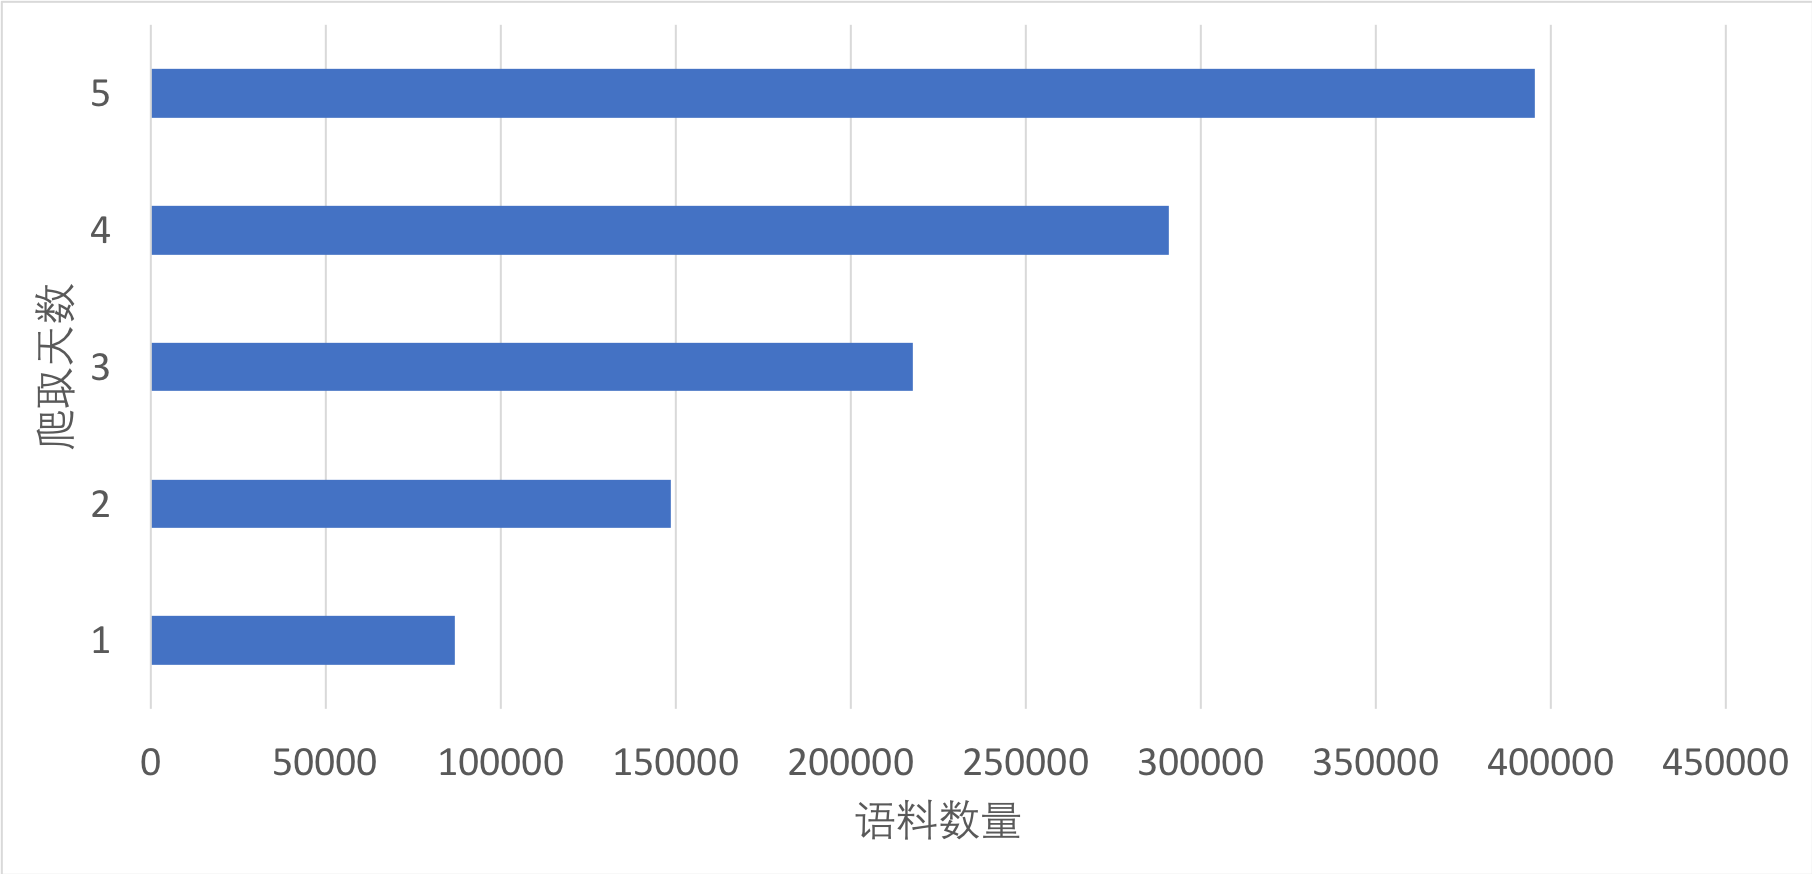
\includegraphics[scale=0.5]{picture/spider_data.png}
    \caption{新闻标题数据增长}
    \label{spider_data_chart}
\end{figure}
为了验证爬虫模块的可靠性和稳定性,以及给后续分类模块提供真实的语料数据,
爬虫网络设置了3个分布式节点连续5天对今日头条网站进行数据爬取工作。同时为了
确保原始语料数据分类的准确性,爬虫模块丢弃了今日头条网站中分类为“视频”和“广告”的文本,
因为这两个分类很多时候只代表其内容的性质,并不是从语言上进行分类,加入训练语料会影响模块
对其他分类的判断。系统5天获取的新闻标题数据如图\ref{spider_data_chart}所示。
可以看出,同过代理IP池、动态爬取间隔等方式,爬虫模块能够很好的突破一般网站的反爬虫技术,
持续增量的获取所需数据。但也由于爬取间隔的存在,限制了每天能获取新闻的数量,需要通过其他手段改进。
\subsection{汉字信息库}
汉字信息库用于给词向量/字向量训练算法提供汉字部首信息,系统共搜集了包括繁简体字在内的
总计20880个汉字的偏旁部首信息,基本上覆盖了人们日常交流中使用的所有汉字。部分数据如表\ref{comp_table}所示:
\begin{table}[h]
    \caption{汉字信息库数据}
    \begin{tabular}{|c|c|c|}
        \hline
        汉字 & 偏旁 & 部首 \\
        \hline
        谴 & 遣 & 讠 \\
        \hline
        延 & 止 & 廴 \\
        \hline
        叛 & 半反 & 又 \\
        \hline
        蘔 & 穎 & 艹 \\
        \hline
    \end{tabular}
    \label{comp_table}
    \end{table}
\subsection{分类测试结果}
模型训练子系统根据第四章的网络结构与相关参数,在每天爬取的新闻标题数据上训练短文本分类网络。
并抽取300条实时新闻,通过系统的分类子系统对其进行测试。测试指标采用了\label{test_fun}小节
介绍的准确率与召回率,计算公式如\label{accuracy}和\label{recall}所示。

图和展示了系统连续5天的准确率与召回率统计,可以看出,准确率整体上保持了一个很高的水准,
而与之相比,系统前期的召回率则非常低,这主要是由于开始系统语料库中新闻语料数据较少,
特别每一类的语料数量非常不均衡,出现次数最少的几类语料(如“时尚”、“游戏”等)甚至
只占总体语料的10\%~15\%,极大的影响了系统在这些类别上的分类效果。
随着爬虫模块搜集的各类语料逐渐增多,召回率也逐步提升,说明通过系统的不断运行,
分类模型的可靠性能够不断提升,最终趋于稳定。同时对于包含新词的语料,虽然初次分类时会由于
预处理模块将其忽略,导致错误分类,但随着语料的补充与完善,系统能够在之后的训练中将其吸收,
得到正确的结果。
\section{本章小节}
本章主要设计并实现了一个短文本分类服务系统。首先对系统的整体架构及运行流程进行了简要描述,
然后对系统中的重要功能模型进行了进一步的介绍。最后针对今日头条网站进行测试,验证了系统的正确性和有效性。
    \chapter{全文总结和展望}
\section{全文总结}
随着我国互联网市场的不断扩大,
网络上充斥了大量有价值或无价值的文本信息,同时由于移动互联设备的逐渐普及,
这些文本信息半数以上以短文本的形式存在。文本分类技术作为自然语言处理的基础技术,
能够有效的理解和梳理这些短文本信息,为后续的文本挖掘工作提供坚实的基础,在
学术研究与商业应用领域都有广泛的使用,具备广阔的应用前景。

本文主要研究了深度学习在中文短文本分类方面的应用,通过研究汉字字词和部首语义上的联系,
以及改进字/词向量模型和特征提取网络,实现了一个新型的文本分类网络模型
,并结合实际场景,构建了一个短文本分类
服务系统。本文的主要贡献如下:
\begin{enumerate}
    \item 对文本分类技术的发展进行了大致介绍,简述了传统文本分类技术的发展现状,
    并对深度学习下的自然语言处理技术进行了简要描述。
    \item 分析了中文词语和词语中包含汉字及相关部首在语义上的内在联系,在CBOW词向量模型的基础
    上引入了汉字和偏旁部首的语义信息,结合部首转换技术,构造了一种新的词向量训练模型,使得训练出的词向量更加切合中文文本,
    具有更强的语义相关性。
    \item 在词向量模型的基础上提出了另一个字向量模型,利用汉字部首的语义信息训练中文字向量,
    让语义上有联系的汉字能够在向量空间中更加靠近,补充了词向量模型的不足。
    \item 结合卷积神经网络与循环神经网络,通过k-max池化与双向循环神经网络技术,
    设计了一个新的特征提取网络。并引入Attention Model技术,让网络能够专注分类特征的提取,
    整体上提升了特征向量质量。
    \item 结合字向量与词向量的文本数据,设计了双通道的短文本分类模型,从两个不同的文本表示中同时提取文本特征,
    极大的丰富了输入短文本的文本信息,有效提升了分类结果,
    并通过与其他同类模型的对比实验,证明了模型的可行性。
    \item 综合本文设计的词/字向量模型与分类网络,结合网络爬虫与WEB服务等模块,实现了一个
    基于网络数据的中文短文本分类服务系统,为外部用户提供持续可靠的短文本分类服务。
\end{enumerate}
\section{后续工作展望}
本文的重点在于寻找一个适合中文短文本的分类模型,由于时间有限,其中仍然有一些改进空间:
\begin{enumerate}
    \item 卷积神经网络与循环神经网络近几年在深度学习领域都有很大发展,可以考虑
    使用其他的网络结构模型改进本文设计的卷积循环特征提取网络,
    如用GRU(Gated Recurrent Unit,门控循环单元)替换LSTM。
    \item 可以使用其他Attention Model的实现方式来筛选文本特征向量,
    通过更复杂的方式获得特征权重,从而进一步优化特征向量。
    \item 本文最后实现的中文短文本分类服务系统,虽然测试有效,但还有很多地方可以
    改进,比如增加更复杂的爬虫管理模块、提升系统计算效率、增加用户管理功能模块等,
    逐步提升系统性能,进一步完善系统功能。
\end{enumerate}

    \thesisacknowledgement
    白驹过隙,时光流逝,又到了毕业的时候了,短短的生活校园生活即将结束,回顾
    整个研究生时光取得的成绩和知识,我由衷的感到满足与幸福。这一切离不开自己的努力与
    坚持,更离不开老师的谆谆教导和同学们的关怀。
    
    在攻读硕士学位期间,首先衷心感谢我的导师陈峥,他为人和善,知识深厚,在
    我学习和生活的方方面面都给与了我指导和帮助,让我获益良多。在项目中给了我们很多的锻炼的机会,
    培养了我们思考和解决工程实践问题的能力。
    在生活上,老师和蔼教人,让我感受良多,获益匪浅。
    每一个细枝末节也在潜移默化中影响和帮助到我面对以后的人生和生活,将使我受益终身。

    我同时也要感谢张婷和刘军在教研室对师弟的指导和关怀,
    让我能更好的融入这个教研室的大集体生活环境,
    同时也让我的研究生生活变得更加精彩,
    指引我在科研的道路上前行,以及在我论文上的指导和建议。

    同时也要感谢三位室友卢震宇,王大帅,徐文龙在研究生学习期间的生活陪伴,因为有了你们,让我的生活变得丰富有趣,
    感谢我的父母,一直以来对我的支持和鼓励,让我能够勇敢地面对一个又一个困难。

    最后,对参加这次论文评审和检查的老师们表示由衷的感谢。

    

    \thesisloadbibliography[nocite]{reference}

    \thesisloadachievement{publications}
\end{document}
